\documentclass[a4paper,12pt,landscape]{article}
\usepackage{multicol}
\usepackage{calc}
\usepackage{ifthen}
\usepackage[a4paper, landscape]{geometry}
\usepackage{amsmath,amsthm,amsfonts,amssymb}
\usepackage{color,graphicx,overpic}
\usepackage{hyperref}
\usepackage{soul} %for highlight
\usepackage{xcolor} %color definition
\usepackage{sectsty} %change section color
\usepackage{tabulary} %better table
% type codes
\usepackage{listings}
\usepackage{xcolor}

\definecolor{codegreen}{rgb}{0,0.6,0}
\definecolor{codegray}{rgb}{0.5,0.5,0.5}
\definecolor{codepurple}{rgb}{0.58,0,0.82}
\definecolor{backcolour}{rgb}{0.95,0.95,0.92}

\lstdefinestyle{mystyle}{
    backgroundcolor=\color{backcolour},
    commentstyle=\color{codegreen},
    keywordstyle=\color{magenta},
    numberstyle=\tiny\color{codegray},
    stringstyle=\color{codepurple},
    basicstyle=\ttfamily\footnotesize,
    breakatwhitespace=false,
    breaklines=false,
    captionpos=b,
    keepspaces=false,
    numbers=left,
    numbersep=5pt,
    showspaces=false,
    showstringspaces=false,
    showtabs=false,
    tabsize=2
}

\lstset{style=mystyle}

\pdfinfo{
  /Title (ST3131 Regression Analysis.pdf)
  /Creator (Ling)
  /Subject (Regression Analysis)}

% This sets page margins to .5 inch if using letter paper, and to 1cm
% if using A4 paper. (This probably isn't strictly necessary.)
% If using another size paper, use default 1cm margins.
\ifthenelse{\lengthtest { \paperwidth = 11in}}
    { \geometry{top=.5in,left=.5in,right=.5in,bottom=.5in} }
    {\ifthenelse{ \lengthtest{ \paperwidth = 297mm}}
        {\geometry{top=.5cm,left=.5cm,right=.5cm,bottom=.5cm} }
        {\geometry{top=.5cm,left=.5cm,right=.5cm,bottom=.5cm} }
    }

% Turn off header and footer
\pagestyle{empty}

% Redefine section commands to use less space
\makeatletter
\renewcommand{\section}{\@startsection{section}{1}{0mm}%
                                {-1ex plus -.5ex minus -.2ex}%
                                {0.5ex plus .2ex}%x
                                {\normalfont\large\bfseries\color{red}}}
\renewcommand{\subsection}{\@startsection{subsection}{2}{0mm}%
                                {-1explus -.5ex minus -.2ex}%
                                {0.5ex plus .2ex}%
                                {\normalfont\normalsize\bfseries\color{blue}}}
\renewcommand{\subsubsection}{\@startsection{subsubsection}{3}{0mm}%
                                {-1ex plus -.5ex minus -.2ex}%
                                {1ex plus .2ex}%
                                {\normalfont\small\bfseries\color{violet}}}
\makeatother

% Define BibTeX command
\def\BibTeX{{\rm B\kern-.05em{\sc i\kern-.025em b}\kern-.08em
    T\kern-.1667em\lower.7ex\hbox{E}\kern-.125emX}}

% Don't print section numbers
\setcounter{secnumdepth}{0}


\setlength{\parindent}{0pt}
\setlength{\parskip}{0pt plus 0.5ex}

%My Environments
\newtheorem{example}[section]{Example}
% -----------------------------------------------------------------------

\begin{document}
\raggedright
\footnotesize
\begin{multicols}{3}


% multicol parameters
% These lengths are set only within the two main columns
\setlength{\columnseprule}{0.25pt}
\setlength{\premulticols}{1pt}
\setlength{\postmulticols}{1pt}
\setlength{\multicolsep}{1pt}
\setlength{\columnsep}{2pt}

\begin{center}
     \Large{\underline{ST3131 Regression Analysis}} \\
     {Lingjie, \today}
\end{center}

\section{ATQ}
\subsubsection{Comment on relationship using Scatter Plot}
\begin{enumerate}
    \item There is/isn't a     
    \item positive/ negative     
    \item linear/ non-linear relationship between $x$ and $y$
    \item with a constant/ non constant Variance
\end{enumerate}

\subsubsection{Fit a linear model}
\begin{enumerate}
    \item Write down fitted model
        \subitem $\hat y = \hat\beta_0 + \hat\beta_1 X_1 + \hat\beta_2 I(X_2 = 1)$
    \item Note: if cat var, write $I(X=\text{Type A})$
\end{enumerate}

\subsubsection{Test model}
\begin{enumerate}
    \item Single regressor: t-test, Multiple regressors: F-test
    \item State $H_0, H_1$
    \item Find t-stat/ F-stat, p-value
    \item Conclude reject/ do not reject $H_0$
\end{enumerate}

\subsubsection{Comment on model Fit}
\begin{enumerate}
    \item $R^2$ is large/ small
    \item F-test is significant/ not significant
\end{enumerate}

\subsubsection{Checking on assumptions}
\begin{enumerate}
    \item Residual plot shows residuals randomly scattered/ some trend about 0, a linear model is sufficient/ insufficient
    \item Residuals plot shows constant/ non constant variance
    \item Standardised residuals shows there are/ no outliers
    \item Residual Normal probability plot shows residuals violate/ does not violate normality assumption
    \item VIF is small suggesting there is/ no multicollinearity
\end{enumerate}

\section{Hypothesis testing}
Statistical Inference: using probability to quantify how plausible a value for a parameter is

\begin{enumerate}
  \item{Assumptions}\\
      \begin{itemize}
          \item Randomised data
          \item Required sample size
          \item Shape of distribution
          \item Note: transformed regressor need to be transformed back
      \end{itemize}

  \item{Hypothesis}
  \begin{itemize}
    \item $H_0 :=$ null hypothesis, represents no effect\\
    \item $H_1 :=$ alternative hypothesis, effect of some type\\
    \item $H_1: p > 0.5, H_1: p < 0.5 :=$ one-sided alternative hypothesis\\
    \item $H_1: p \neq 0.5 :=$ two-sided alternative hypothesis\\
    \item Note: $H_0, H_1$ cannot have any overlap
  \end{itemize}

  \item{Test Statistics}
  \begin{itemize}
    \item Describes how far that point estimate falls from the parameter value given in $H_0$\\
    \item Required: 
        \subitem 1. value in the sample, 
        \subitem 2. parameter value in $H_0$
  \end{itemize}

		\item{$p$-value}
			\begin{itemize}
				\item Probability in sampling distribution that test statistic assumes a value more extreme (tail probability) than observed\\
				\item Small $p$-value, either reject $H_0$ or sample is not representative of the population\\
				\item Note: for $F$-test, it is only the right tail
			\end{itemize}

		\item{Conclusion}\\
			Reports the $p$-value, and summarises how much evidence there is against $H_0$

	\end{enumerate}

		\subsubsection{Checking Normality using QQ-plots}
		QQ-plots: standardised sample quantiles vs theoretical quantiles of a $N(0, 1)$ distribution. When compared to the straight line:
        \begin{lstlisting}[language=R]
qqnorm(X)  # qq plot
qqline(X)  # line
        \end{lstlisting}
			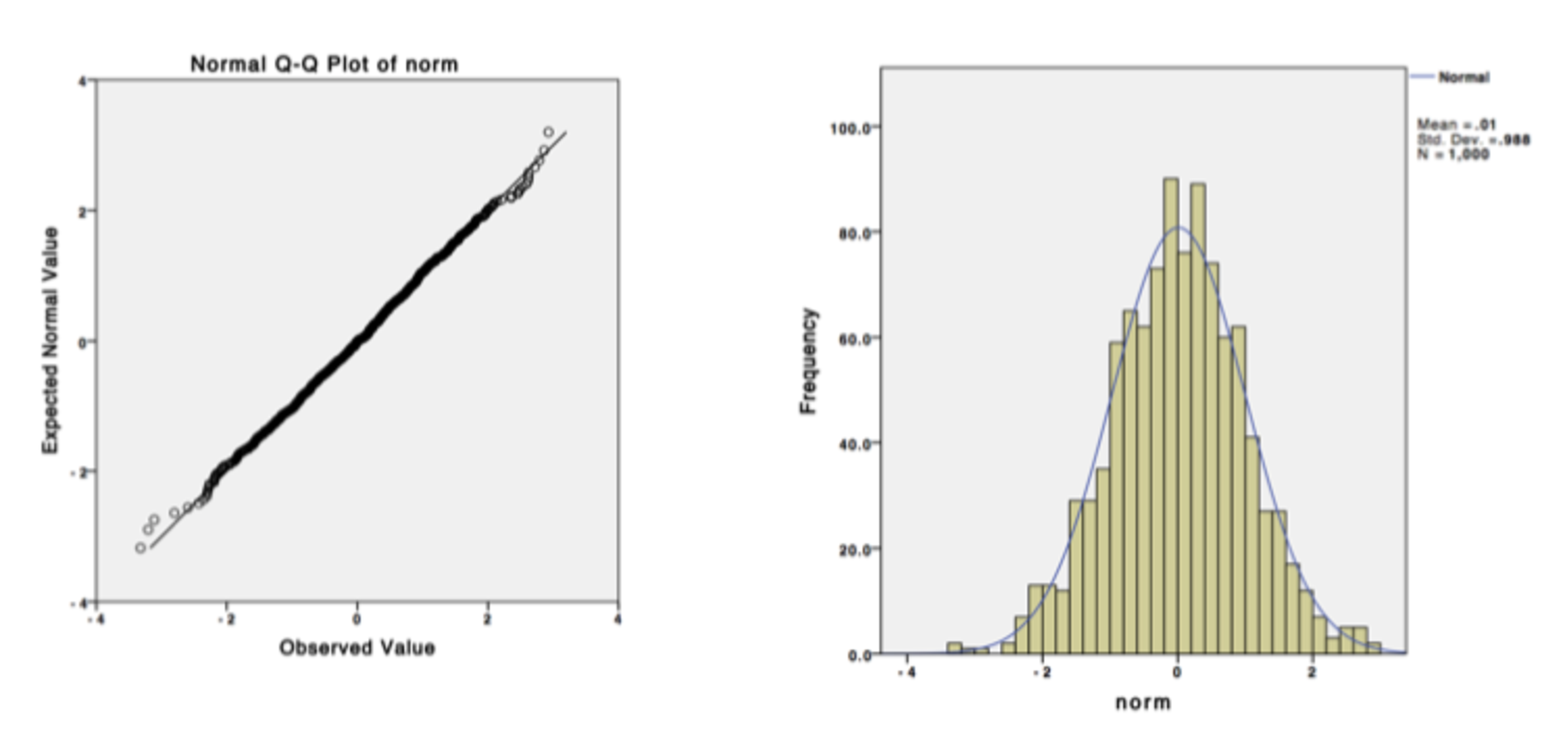
\includegraphics[width=\linewidth]{figures/QQ-plot-Data-From-Normal-Distribution}
			\begin{itemize}
				\item Left tail shorter, Right tail longer: Right-skewed
					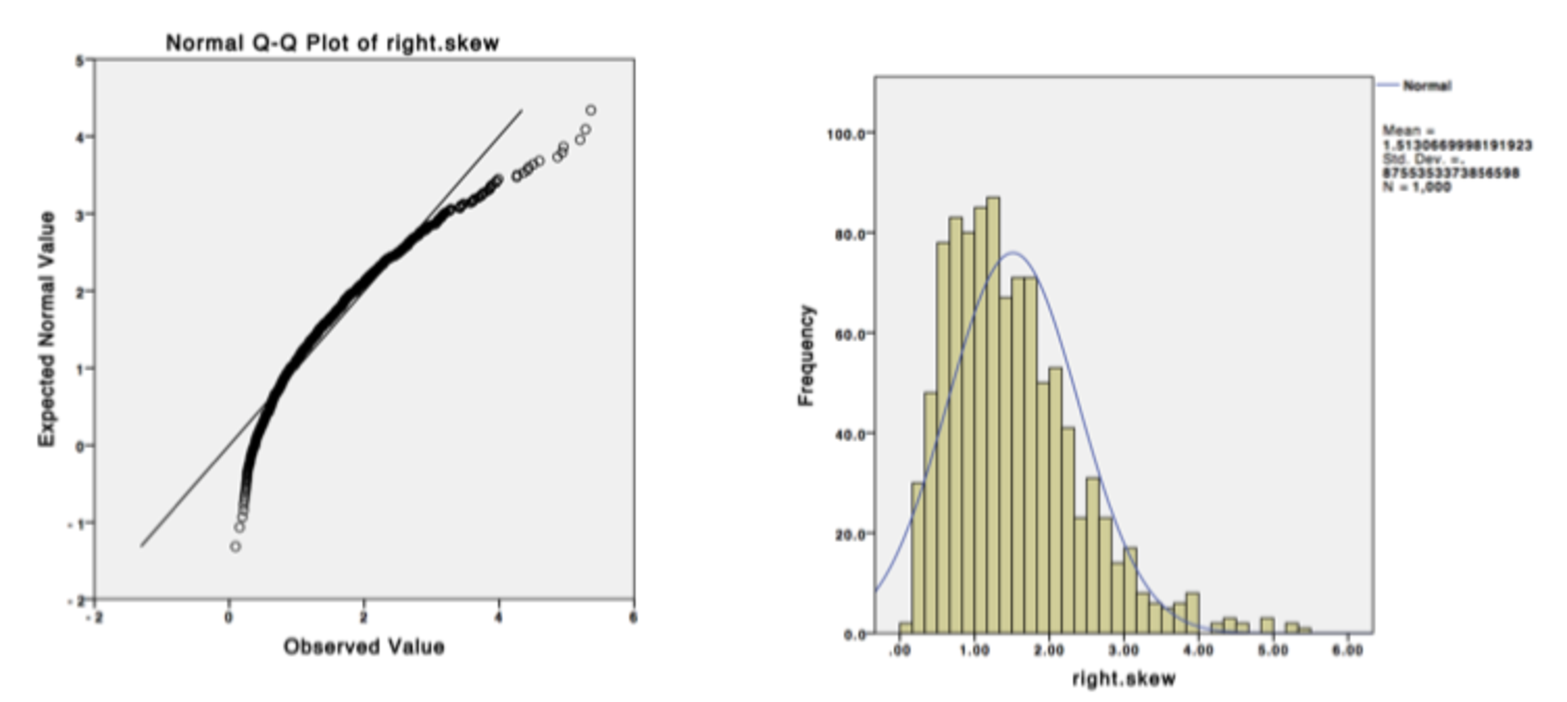
\includegraphics[width=\linewidth]{figures/QQ-plot-Data-From-Right-Skewed-Distribution}
				\item Left tail longer, Right tail shorter: Left-skewed
					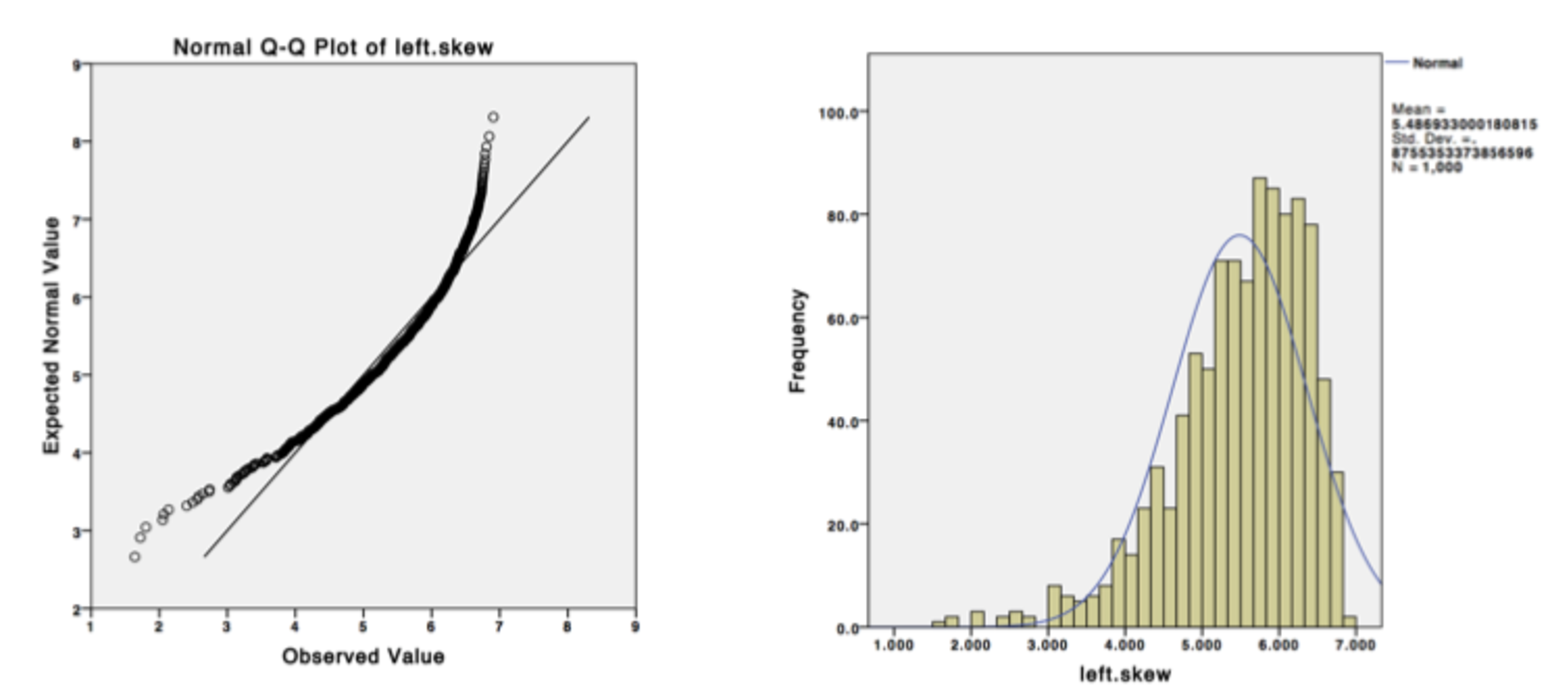
\includegraphics[width=\linewidth]{figures/QQ-plot-Data-From-Left-Skewed-Distribution}
				\item Both tails longer
					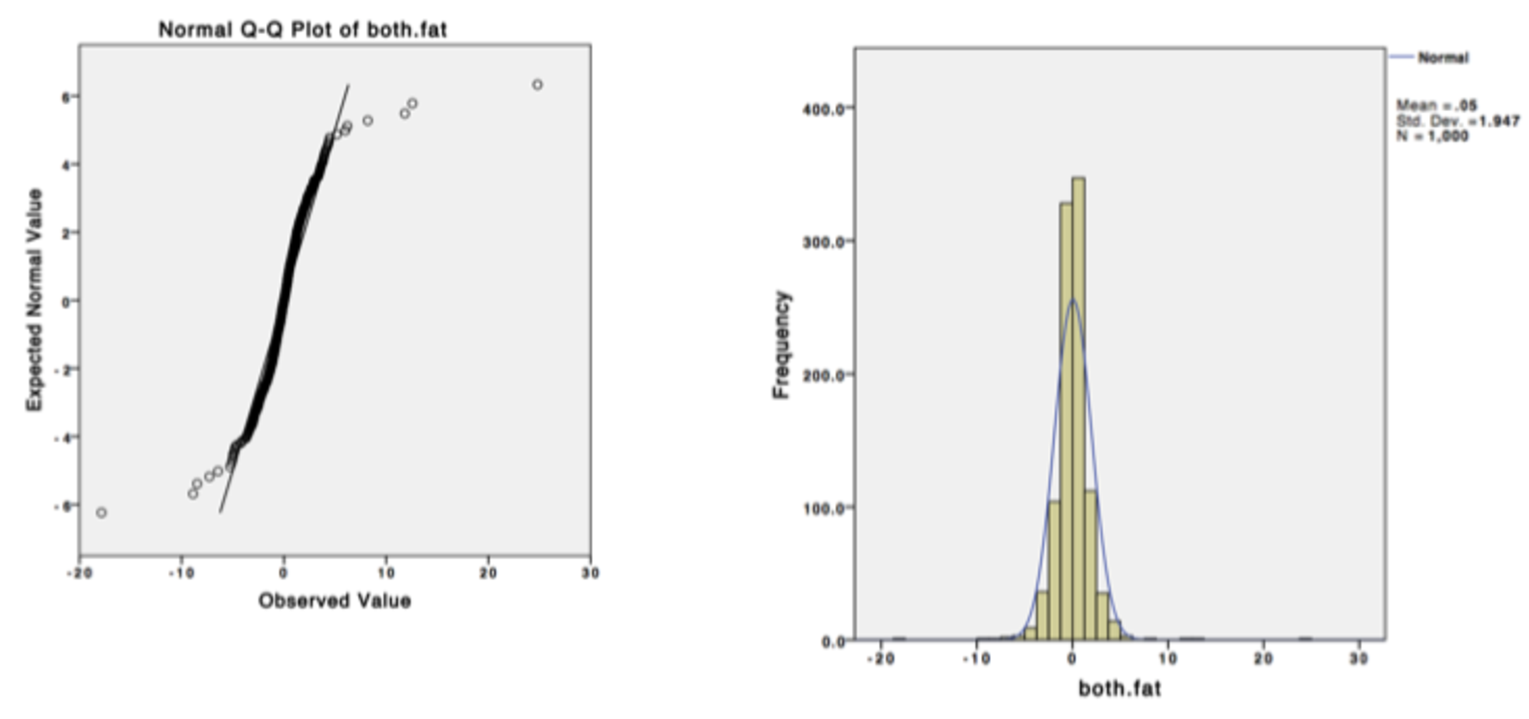
\includegraphics[width=\linewidth]{figures/QQ-plot-Both-Tails-Longer-Than-Normal}
				\item Both tail shorter
					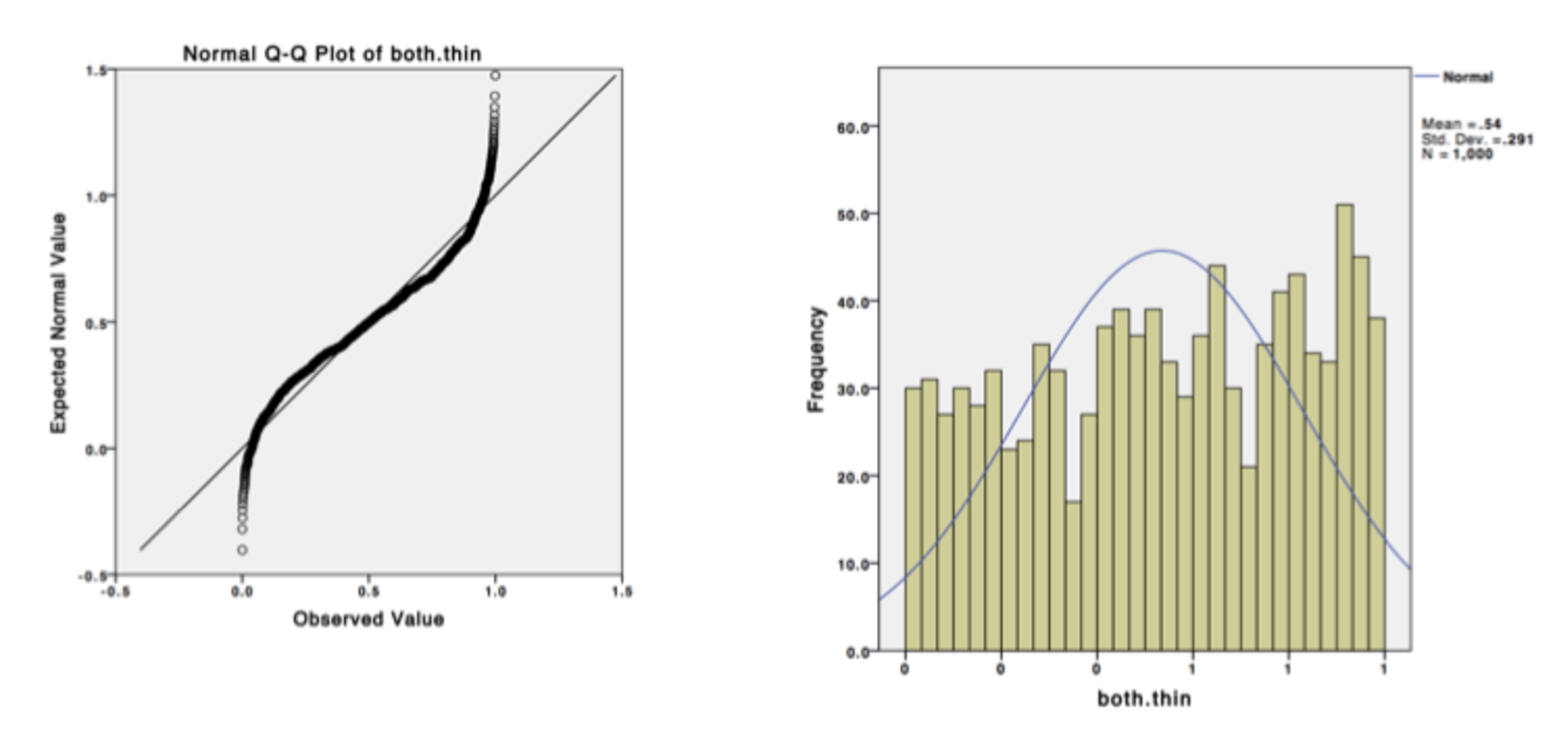
\includegraphics[width=\linewidth]{figures/QQ-plot-Both-Tails-Shorter-Than-Normal}
				\item Right tail is below: longer than Normal
				\item Right tail is above: shorter than Normal
				\item Left tail is below: shorter than Normal
				\item Left tail is above: longer than Normal
			\end{itemize}
		Alternative method: Anderson-Darling test\\ $H_0:$ data is normal vs $H_1:$ data is not normal

	\subsection{Hypothesis Testing for Means}
		$\mu:=$ population mean

		\subsubsection{One-Sample t-Test for Means}
			\begin{enumerate}
				\item{Assumption}
					\begin{itemize}
						\item variable measured is quantitative
						\item data obtained through randomization
						\item population distribution is approximately Normal, crucial when $n$ is small
					\end{itemize}
				\item{Hypothesis}\\
					$H_0: \mu = \mu_0$,    $H1: \mu \neq \mu_0$
				\item{Test Statistics}\\
					point estimate: $\bar X$\\
                    $T = \frac{\bar X - \mu_0}{s/\sqrt{(n)}}\sim t_{n-1}$
				\item{$p$-Value}\\
					\begin{lstlisting}[language=R]
t.test(data, mu=0) # default: 2-sided
					\end{lstlisting}
				\item{Conclusion}\\
					Report and interpret $p$-value in the context of the experiment
			\end{enumerate}

		\subsubsection{Confidence Interval}
		95\% Confidence Interval for the Mean\\
		$\bar X \pm t_{n-1, 0.975} \times s/\sqrt{n}$\\
		$\bar X \pm t_{n-1, 0.975} \times SE(\bar X)$

	\subsection{Comparing Means}

		\subsubsection{Tests for Comparing Two Group Means}
			Not the focus of this module, but we can use $H_0: \mu_1 = \mu_2 \Rightarrow \mu_1 - \mu_2 = 0$ and apply $t$-test

		\subsubsection{ANOVA}
			Let $I:=$ num of groups and $J:=$ num of obs in each group
			\begin{enumerate}
				\item Assumption\\
					errors are normally distributed
				\item Hypothesis\\
					$H_0: \beta_1 = \beta_2 = \cdots = \beta_I = 0$
				\item Test Statistics\\
					$F = \frac{SS_B / (I-1)}{SS_W [I(J-1)]}\sim F_{I-1, I(J-1)}$\\
				\item $p$-value\\
					reject $H_0$ if $F> F_{I-1, I(J-1)}(\alpha)$\\
					\hl{Note: F-stat test only on the right tail, even if test
                    is 2-sided}
				\item Conclusion
			\end{enumerate}

\section{Linear Regression}
	\begin{lstlisting}[language=R]
model <- lm(y~x+I(x^2)+log(x), data=data)
summary(model) # regression results
anova(model) # ANOVA table
predict(model, data.frame(x1=x),
	interval="confidence", level=0.95)
predict(model, data.frame(x1=x),
	interval="prediction", level=0.95)
qt(alpha/2, df) # quantile
pt(t0, df)  # probability
	\end{lstlisting}

	\begin{tabulary}{\linewidth}{l @{ : } L}
    Population model & $\bold{y_{n\times 1}} = \bold{X_{n\times p}\beta_{p\times 1} + \epsilon_{n\times 1}}$\\
		Fitted model & $\hat y = \hat\beta_0 + \hat\beta_1x + \hat\beta_2x^2$\\
		Hat matrix ($\bold H$) & $\bold{\hat y} = \bold X \bold{\hat\beta} = \bold X (\bold X^T \bold X)^{-1}\bold{X^T}\bold y$\\
		& $\bold H \bold y$\\
		Sample regression model & $y_i = \beta_0 + \beta_1x_i + \epsilon_i$\\
	\end{tabulary}

	Note: \\
    linearity refers to parameters (coefficients)\\
    fitted model has no error term\newline

	Main Objective of Regression Analysis
	\begin{itemize}
		\item model fitting\\
			estimate unknown parameters (OLS, MLE)
		\item model adequacy checking\\
			validate appropriateness of the model
	\end{itemize}

		\subsubsection{Notations}
			\begin{tabulary}{\linewidth}{l @{ := } L}
				$\epsilon$ & random (uncorrelated) error term\\
				& $E(\epsilon)=0$ and $Var(\epsilon) = \sigma^2$\\
				$y_i$ & $i$th dependent (response/target/output) variable\\
				$x_{ij}$ & independent (predictor/input/covariate/regressor)\\ &$i$th observation of regressor $x_j$\\
				$k$ & num of regressors, excl $\beta_0$\\
				$p$ & $k+1$, incl $\beta_0$\\
				$\beta_0$ & intercept, always assumed exist\\
				$\beta_i$ & slope\\
				$E(y|x)$ & $\mu_{y|x} = E(\beta_0 + \beta_1 x + \epsilon | x) = \beta_0 + \beta_1 x$\\
				$Var(y|x)$ & $\sigma^2_{y|x} = Var(\beta_0 + \beta_1x + \epsilon | x) = \sigma^2$
			\end{tabulary}


	\subsection{Estimation of the Model Parameters}

		\subsubsection{Simple regression}
			Objective:
			\begin{align*}
				\min S(\beta_0, \beta_1) = \sum_{i=1}^n\epsilon_i^2 = \sum_{i=1}^n(y_i-\beta_0-\beta_1x_i)^2
			\end{align*}
        \hl{Solution:}
			\begin{align*}
				\hat\beta_0 &= \bar y - \hat\beta_1 \bar x\\
				\hat\beta_1 &= \frac{\sum_{i=1}^ny_ix_i - \frac{(\sum_{i=1}^ny_i)(\sum_{i=1}^nx_i)}{n}}{\sum_{i=1}^nx_i^2-\frac{(\sum_{i=1}^nx_i)^2}{n}} \\
				&= \frac{Cov(X, Y)}{Var(X)} = \frac{S_{xy}}{S_{xx}}\\
                Var(y) &= \frac{SS_T}{n-1}\\
                Var(X) &= \frac{S_{xx}}{n-1}
			\end{align*}
			Notation:
			\begin{align*}
				S_{xy} &= \sum_{i=1}^ny_ix_i - \frac{(\sum_{i=1}^ny_i)(\sum_{i=1}^nx_i)}{n} = \sum_{i=1}^ny_i(x_i-\bar x)\\
				S_{xx} &= \sum_{i=1}^nx_i^2-\frac{(\sum_{i=1}^nx_i)^2}{n} = \sum_{i=1}^n(x_i - \bar x)^2
			\end{align*}

		\subsubsection{Multiple regression}
			$\bold y = \begin{bmatrix} y_1 \\ y_2 \\ \vdots \\ y_n \end{bmatrix}_{n\times 1}
			\bold X = \begin{bmatrix} 1 & x_{11} & x_{12} & \cdots &  x_{1k} \\
			1 & x_{21} & x_{22} & \cdots & x_{2k} \\
			\vdots & \vdots & \vdots &  &\vdots \\
			1 & x_{n1} & x_{n2} & \cdots & x_{nk} \end{bmatrix}_{n\times p}$\\
			$\bold\beta = \begin{bmatrix}\beta_0 \\ \beta_1 \\ \vdots \\ \beta_k \end{bmatrix}_{p\times 1}
			\bold\epsilon = \begin{bmatrix}\epsilon_1 \\ \epsilon_2 \\ \vdots \\ \epsilon_n \end{bmatrix}_{p\times 1}$\\

			\ \\Objective:
			\begin{align*}
				\min S(\bold \beta) &= \sum_{i=1}^n\epsilon^2 = \bold\epsilon^T\bold\epsilon = (\bold y - \bold X \bold\beta)^T(\bold y - \bold X \bold\beta)\\
				&=\bold y ^T \bold y - 2\bold\beta^T \bold X ^T \bold y + \bold \beta^T \bold X^T \bold X \bold \beta
			\end{align*}
			Note: $(\bold\beta^T\bold X^T \bold y)_{1\times 1}$ is a scalar

			\ \\Solution:
			\begin{align*}
				\bold{\hat\beta} = (\bold X^T\bold X)^{-1}\bold X^T \bold y
			\end{align*}
			$(\bold X^T\bold X)^{-1}$ exist $\Leftrightarrow$ regressors are linearly independent

		\subsubsection{Properties of the Least-Squares Estimation}
			Key: unbiased mean + small variance

			$\hat\beta_1 = \frac{S_{xy}}{S_{xx}} = \sum_{i=1}^n\frac{(x_i-\bar x)}{S_{xx}}y_i = \sum_{i=1}^nc_iy_i$\\
			$\because \sum_{i=1}^nc_i=0, \sum_{i=1}^nc_ix_i=1, \sum_{i=1}^nc_i^2=\frac{1}{S_{xx}}$

            \begin{align*}
                E(\hat\beta_1) = \beta_1,~~ & E(\hat\beta_0)=\beta_0\\
                Var(\hat\beta_1) = \frac{\sigma^2}{S_{xx}},~~ & Var(\hat\beta_0) = \sigma^2(\frac{1}{n}+\frac{\bar x^2}{S_{xx}})
            \end{align*}

        \subsubsection{Mean and Variance of $\bold{\hat\beta}$}
            $\because E(\epsilon)=0, (\bold{X^TX})^{-1}\bold{X^TX=I}$\\
            $E(\bold{\hat\beta})=E[(\bold{X^TX})^{-1}\bold{X^Ty}]=E[(\bold{X^TX})^{-1}\bold{X^T}(\bold{X\beta+\epsilon})]
            =E[(\bold{X^TX})^{-1}\bold{X^TX\beta}+(\bold{X^TX})^{-1}\bold{X^T\epsilon}]=\bold{\beta}$

            $Cov(\bold{\hat\beta})=E\left\{[\bold{\hat\beta-E(\hat\beta)}][\bold{\hat\beta-E(\hat\beta)}]^T\right\}_{p\times
            p}$ symmetric matrix\\
            the $j^{th}$ diagonal element is $Var(\hat\beta_i)$ and $(ij)$th
            off-diagonal element is $Cov(\hat\beta_i, \hat\beta_j)$ Hence\\
            $Cov(\hat\beta)=Var(\hat\beta)=Var\left[(\bold{X^TX})^{-1}\bold{X^Ty}\right]=(\bold{X^TX})^{-1}\bold{X^T}Var(\bold{y})\left[(\bold{X^TX})^{-1}\bold{X}^T\right]^T=\sigma^2(\bold{X^TX})^{-1}\bold{X^TX(X^TX)^{-1}}=\sigma^2\bold{(X^TX)^{-1}}$\\
            Denote $\bold{C=(X^TX)^{-1}}$, then
            $Var(\hat\beta_j)=\sigma^2C_{jj}$ and
            $Cov(\hat\beta_i,\hat\beta_j)=\sigma^2C_{ij}$
            \begin{align*}
                E(\bold{\hat\beta}) = \bold{\beta}, &~~Cov(\bold{\hat\beta})=\sigma^2\bold{(X^TX)^{-1}}\\
                Var(\hat\beta_j) = \sigma^2C_{jj}, &~~Cov(\hat\beta_i, \hat\beta_j)=\sigma^2C_{ij}
            \end{align*}

		\subsubsection{Estimation of $\sigma^2$}
			Denote $SS_T = \sum_{i=1}^n(y_i-\bar y)^2$ (not model dependent)
			\begin{align*}
				SS_{Res} &= SS_T - \hat\beta_1S_{xy} \text{(model dependent)}\\
				\sum_{i=1}^ne_i^2 &= \sum_{i=1}^n(y_i-\hat y_i)^2 = \sum_{i=1}^ny_i^2-n\bar y^2 - \hat\beta_1S_{xy}\\
				&= \sum_{i=1}^n(y_i-\bar y)^2 - \hat\beta_1 S_{xy}
			\end{align*}
			$\because E(SS_{Res}) = (n-p)\sigma^2, p:=$ num of regressors (includ $\beta_0$)\\
			$\therefore \hat\sigma^2 = SS_{Res}/(n-p)$, unbiased estimator of $\sigma^2$

			Denote $MS_{Res} = SS_{Res} / (n-p)$, residual mean square\\
			$\hat\sigma :=$ residual standard error or standard error of regression

            \begin{align*}
                \hat\sigma^2 = MS_{Res} = \frac{SS_{Res}}{n-p}
            \end{align*}

        \subsubsection{Estimation of $\sigma^2$, multiple regression}
            $SS_{Res}=\sum_{i=1}^n(y_i-\hat
            y_i)^2=\sum_{i=1}^ne_i^2=\bold{e^Te}$\\
            Sub $\bold{e=y-X\hat\beta}$\\
            $SS_{Res}=\bold{(y-X\hat\beta)^T(y-X\hat\beta)}$\\
        $\bold{=y^Ty-\hat\beta^TX^Ty-y^TX\hat\beta+\hat\beta^TX^TX\hat\beta}$\\
        $\bold{=y^Ty-2\hat\beta^TX^Ty+\hat\beta^TX^TX\hat\beta}$\\
        Since $\bold{X^TX\hat\beta=X^Ty}\Rightarrow
        SS_{Res}=\bold{y^Ty-\hat\beta^TX^Ty}$\\
        $MS_{Res}=\frac{SS_{Res}}{n-p}\Rightarrow
        E(MS_{Res})=\sigma^2\Rightarrow \hat\sigma^2 = MS_{Res}$ is unbiased
        estimator of $\sigma^2$


	\subsection{Hypothesis Testing}
    \begin{align*}
        &y_i \sim N(\beta_0 + \sum_{i=1}^k\beta_j x_{ij}, \sigma^2)\\
        &\bold{\hat\beta} \sim N(\bold{\beta}, \sigma^2\bold{(X^TX)^{-1}}), \hat\beta_j \sim N(\beta_j, \sigma^2C_{jj})
    \end{align*}
		Assumption:
		\begin{itemize}
			\item $x, y$ shares linear relationship
			\item uncorrelated errors with $E(\epsilon)=0$ and $Var(\epsilon) = \sigma^2$
			\item $\epsilon_i \sim N(0, \sigma^2)$\\
				Note: for each sub-population, they have the same variance
		\end{itemize}

		\subsubsection{$t$ test: Individual Regression Coefficient}
		$H_0: \beta_1 = 0, H_1: \beta_1 \neq 0$
        \begin{align*}
            t_0 &= \frac{\hat\beta_1}{\sqrt{MS_{Res}/S_{xx}}} = \frac{\beta_j}{\sqrt{\hat\sigma^2C_{jj}}}=\frac{\hat\beta_1}{se(\hat\beta_1)} \sim t_{n-p}
    \end{align*}
    $C_{jj}$ is diagonal element $\bold{(X^TX)^{-1}} \Leftrightarrow \hat\beta_j$

		$H_0: \beta_0 = 0, H_1: \beta_0 \neq 0$
        \begin{align*}
            t_0 = \frac{\hat\beta_0}{se(\hat\beta_0)} = \frac{\hat\beta_0}{\sqrt{MS_{Res}(1/n+\bar x^2/S_{xx})}} \sim t_{n-p}
    \end{align*}
        rejected $H_0$ if $|t_0|>t_{n-k-1(\alpha/2)}$\\
        Note: the test is given other regressors in the model

		\subsubsection{$F, t$ test: Significance of Regression}
		$H_0: \beta_1 = \beta_2 = \cdots \beta_j = 0, H_1:$ at least 1 $\beta_i \neq 0$
        \begin{align*}
            F = \frac{SS_R / k}{SS_{Res} / (n-k-1)} = \frac{MS_R}{MS_{Res}}\sim F_{df_{SS_R}, df_{SS_{Res}}}
    \end{align*}
        Reject $H_0$ if $F_0 > F_{k, n-k-1}(\alpha)$\\

        \hl{ANOVA table}
			\begin{tabulary}{\linewidth}{L | L | l | l | l}
				\hline
				Source of Variation & Sum of Squares & DF & MS & $F_\alpha$\\
				\hline
				Regression & $SS_R$ & k & $MS_R$ & $MS_R/MS_{Res}$\\
				Residual & $SS_{Res}$ & n-p & $MS_{Res}$\\
				Total & $SS_T$ & n-1\\
				\hline
			\end{tabulary}

		$SS_T = SS_R + SS_{Res}$, $SS_R$ is model dependent\\
		$\sum_{i=1}^n(y_i-\bar y)^2 = \sum_{i=1}^n(\hat y_i - \bar y)^2 + \sum_{i=1}^n(y_i - \hat y_i)^2$
    \subsubsection{Extra-sum-of-squares Method}
    Useful to select a subset of regressors\\
    Extra-sum-of-square due to $\bold{\beta_2}: SS_R(\beta_2|\beta_1)=SS_R(\beta)-SS_R(\beta_1)$ with $df=r$\\
    $H_0: \beta_2 = 0, H_1: \beta_2 \neq 0$
    \begin{align*}
        F_0 = \frac{SS_R(\beta_2|\beta_1)/r}{MS_{Res}}\sim F_{r, n-p}
    \end{align*}
    Note: in R the order we put regressors matters\\
    \hl{$t^2 = F_0 \sim F_{1, n-p}$}

    \subsubsection{ESS: Orthogonal Col in $\bold{X}$}
    consider $\bold{y = X\beta + \epsilon = X_1 \beta_1 + X_2\beta_2 + \epsilon}$, if $\bold{X_1}\perp\bold{X_2}$, Sum of square and model is the same regardless of order to add in regressors $\Rightarrow$ no need to refit (rare case)

    \subsection{Confidence Intervals}

		\subsubsection{CI on the Regression Coefficients}
			\begin{align*}
				\beta_i \in & ~ \hat\beta_i \pm t_{n-p}(\alpha/2)\times se(\hat\beta_i)\\
				\sigma^2 \in & ~ \left(\frac{{(n-p)}MS_{Res}}{\chi_{n-p}^2(\alpha/2)}, \frac{{(n-p)}MS_{Res}}{\chi_{n-p}^2(1-\alpha/2)}\right)
			\end{align*}

		\subsubsection{CI Estimation of the Mean Response}
		Mean Response: $E(y|x_0)$\\
		$\hat{E(y|x_0)} = \hat\mu_{y|x_0} = \hat\beta_0 + \hat\beta_1 x_0$\\
        $Var(\hat\mu_{y|x_0}) = Var(\hat\beta_0 + \hat\beta_1x_0) = Var(\bar y + \hat\beta_1(x_0-\bar x))$\\ $= \sigma^2\left(\frac{1}{n}+\frac{(x_0-\bar x)^2}{S_{xx}}\right)=\sigma^2\bold{x_0^T(X^TX)^{-1}x_0}$

			\begin{align*}
                &E(y|x_0) \in \hat\mu_{y|x_0} \pm t_{n-p}(\alpha/2)\sqrt{MS_{Res}\left(\frac{1}{n}+\frac{(x_0-\bar x)^2}{S_{xx}}\right)}\\
                &E(y|x_0) \in \hat y_0 \pm t_{n-p}(\alpha/2)\sqrt{\hat\sigma^2\bold{x_0^T(X^TX)^{-1}x_0}}
			\end{align*}

		Note
			\begin{itemize}
				\item CI for $E(y|x_0)$ is a function of $x_0$
				\item interval width minimised at $x_0 = \bar x$ and widens as $|x_0 - \bar x|$ increases
				\item standard error for a CI on mean responses takes into account the uncertainty due to sampling $\Rightarrow$ confidence band is not parallel
			\end{itemize}
			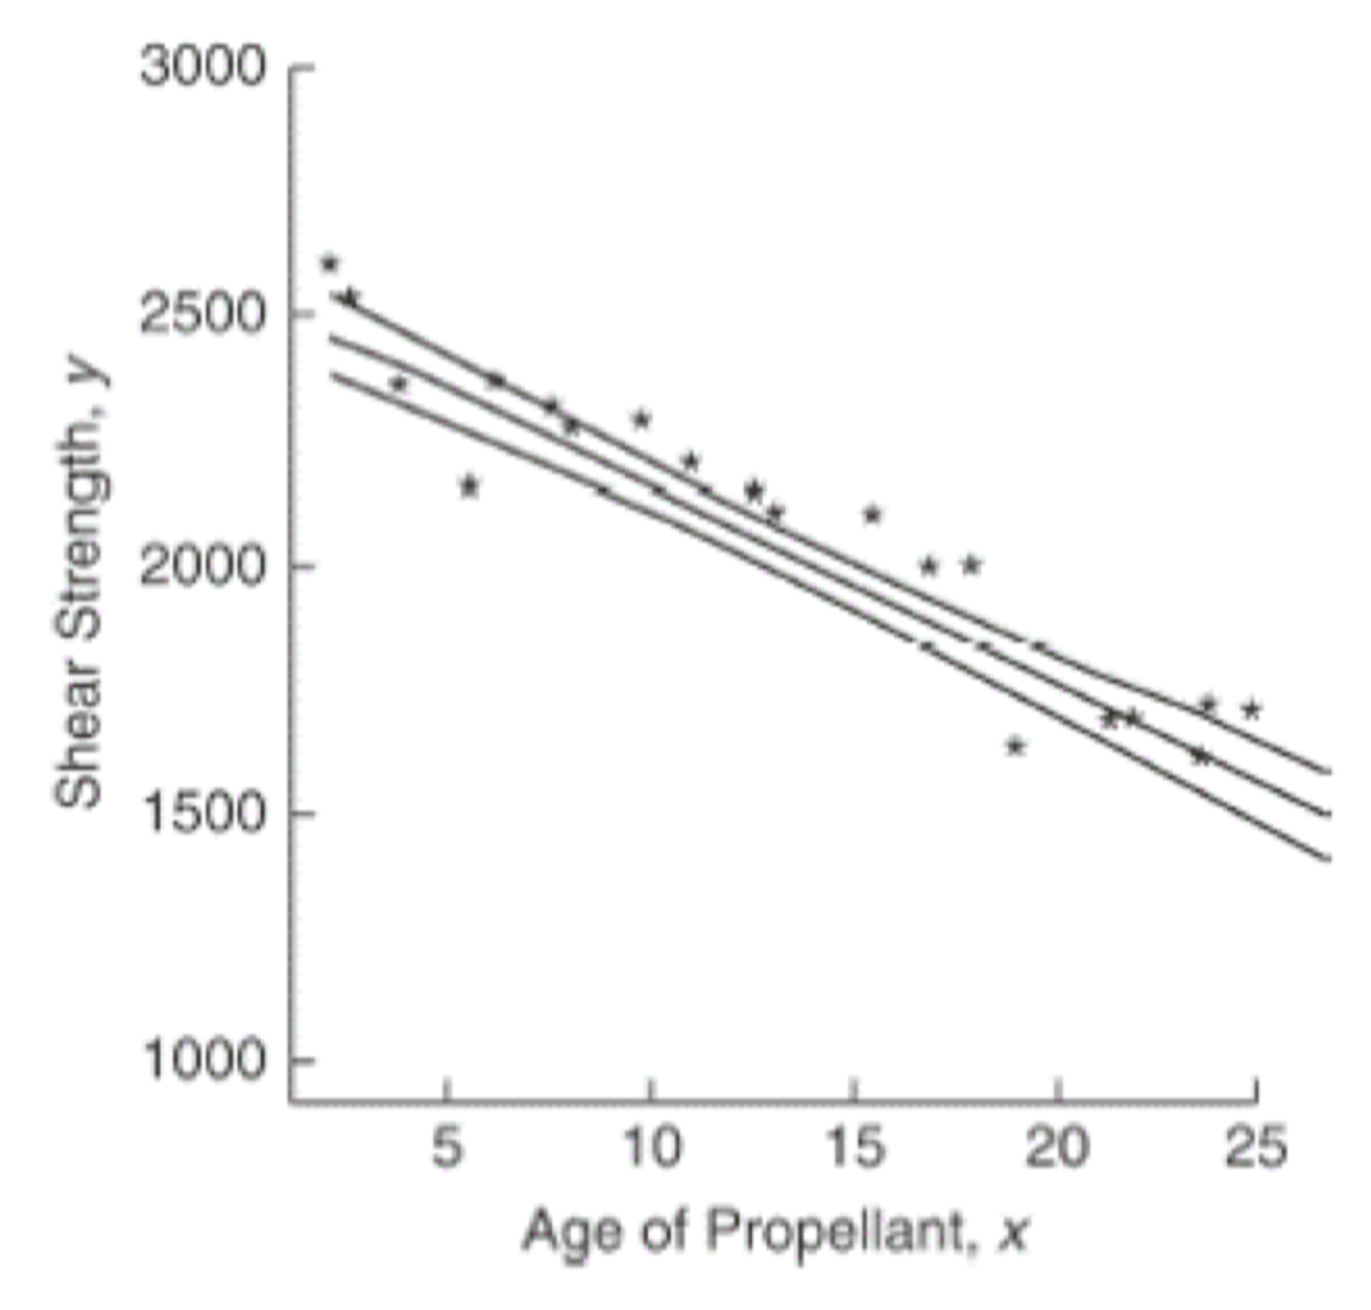
\includegraphics[width=.5\linewidth]{figures/confidence_limits}

        \subsubsection{Simultaneous CI on Regression Coefficients}
        Bonferroni Method, useful when trying to find the joint CI of $\beta_i, \beta_j, i\neq j$\\
        \begin{align*}
            \hat\beta_j \pm t_{n-p}(\alpha/2p)\times se(\hat\beta_j), j \in[0, k]
        \end{align*}


		\subsubsection{Prediction Interval}
        Note: check if $X$ is in the range of dataset\\
		Prediction: $\hat y_0 = \hat\beta_0 + \hat\beta_1 x_0$, let $\psi = y_0 - \hat y_0$\\
		Note: Prediction interval is for the future observation $y_0$ can be obtained, and future observation $y_0$ is independent of our prediction $\hat y_0$

		$Var(\psi) = Var(y_0) - 2 Cov(y_0, \hat y_0) + Var(\hat y_0)$
		$=\sigma^2 + \sigma^2\left(\frac{1}{n}+\frac{(x_0-\bar x)^2}{S_{xx}}\right)$

		\begin{align*}
            &y_0 \in \hat y_0 \pm t_{n-p}(\alpha/2)\sqrt{MS_{Res}\left(1+\frac{1}{n}+\frac{(x_0-\bar x)^2}{S_{xx}}\right)}\\
            &y_0 \in \hat y_0 \pm t_{n-p}(\alpha/2)\sqrt{\hat\sigma^2(1+\bold{x_0^T(X^TX)^{-1}x_0})}
		\end{align*}

		Note: standard error for a prediction interval of a future observation takes into account the uncertainty due to sampling and variability of the individual around the predicted mean.
		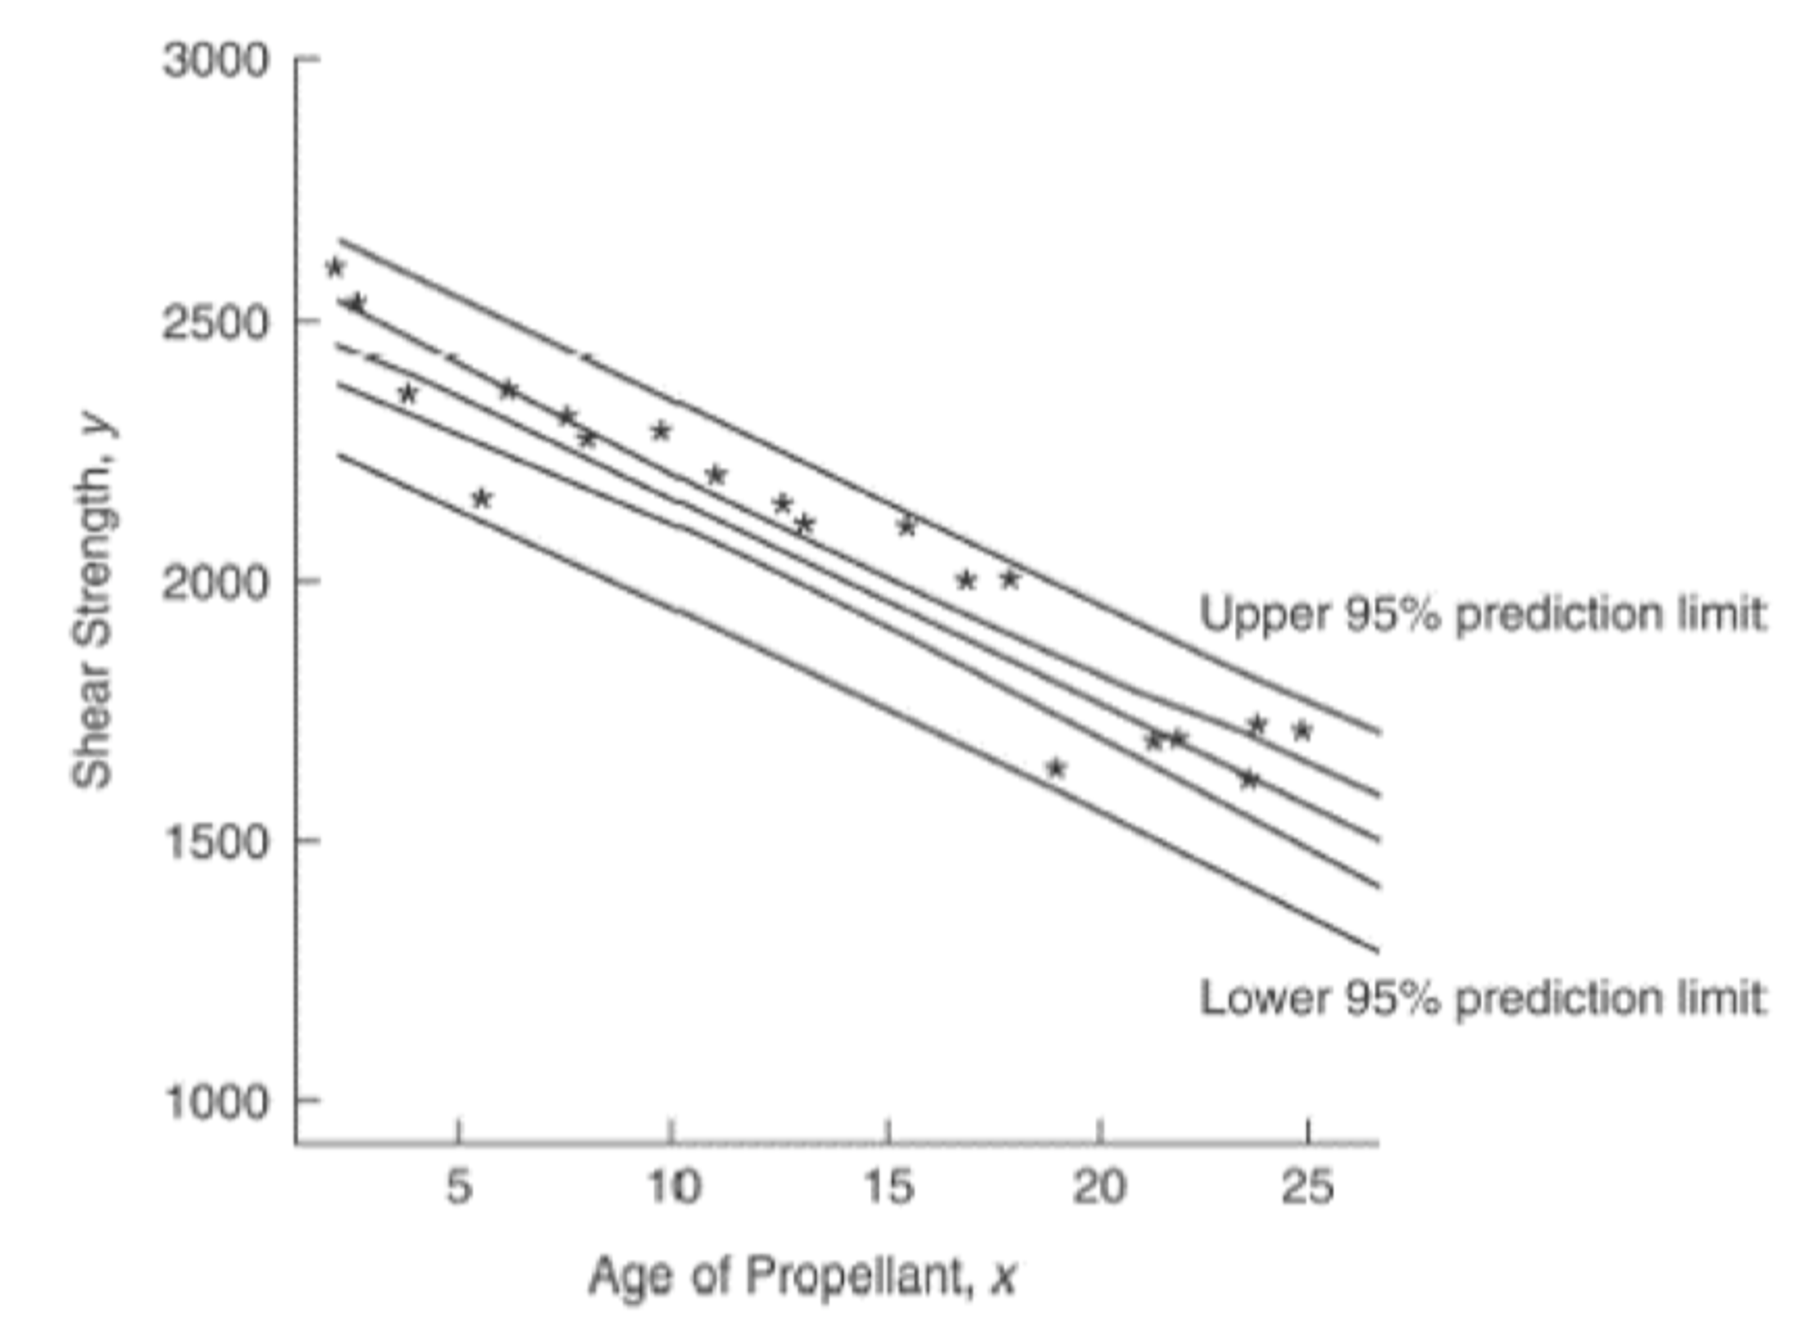
\includegraphics[width=\linewidth]{figures/prediction_interval}

	\subsection{Coefficient of Determination $R^2$}
		\begin{align*}
			R^2 &= \frac{SS_R}{SS_T}=1-\frac{SS_{Res}}{SS_T}\\
			R_{Adj}^2 &= 1-\frac{SS_{Res}/(n-p)}{SS_T/(n-1)}\\
			&= 1-\frac{n-1}{n-p}(1-R^2)\\
            cor(y, \hat y) &= |cor(y, x)|=\sqrt{R^2}
		\end{align*}
		proportion of variation explained by the regressors

	\subsection{Interpretation of Regression Coefficients}

        \subsubsection{First Interpretation}
        changes in mean response $\frac{\partial}{\partial x_i}E(y|X)$

        \subsubsection{Second Interpretation}
        contribution of $x_j$ to $y$ after both $y, x_j$ have been linearly adjusted for all other regressors
        $e_{y, x_1, x_2, \cdots, x_{k-1}} = \beta_ke_{x_k,x_1,x_2,\cdots, x_{k-1}}$

		\subsection{Hidden Extrapolation in Multiple Regression}

        \subsubsection{Regressor Variables Hull (RVH)}
        Using the hat matrix $\bold{H=X(X^TX)^{-1}X^T}$ \\
        and set $\max{h_{ii}}:=h_{max}$\\
        To be within the ellipsoid, $\bold{x^T(X^TX)^{-1}x}\leq h_{max}$\\
        Therefore, the new estimation at point $\bold{x_0^T}=[1, x_{01}, x_{02}, \cdots, x_{0k}]$ will have $h_{00}=\bold{x_0^T(X^TX)^{-1}x_0}$\\
        if $h_{00} > h_{max}$, then the point is a point of extrapolation

		\subsection{Indicator Variables}
        Categorical variables, we assign dummy variables, $\alpha - 1$\\
                $x = \begin{cases}0 & \text{if obs from type A}\\ 1 & \text{if obs from type B}\end{cases} ~~= I(\text{obs from type B})$\\
                Same slope, different intercept for different type\\
                To test for significance of 3 types:
                \begin{align*}
                    H_0:& \beta_2 = \beta_3 = 0\\
                    H_1:& \beta_2 \neq 0 \text{ and/or } \beta_3 \neq 0
                \end{align*}
    \begin{lstlisting}[language=R]
# recode to cat var
data$x11 <- as.factor(data$x11)
    \end{lstlisting}


		\subsection{Interaction Term}
			$y=\beta_0+\beta_1x_1+\beta_2x_2+\beta_3x_1x_2+\epsilon$\\
			$\frac{\delta}{\delta x_1}E(y|x_1, x_2) = \beta_1 + \beta_3x_2$
			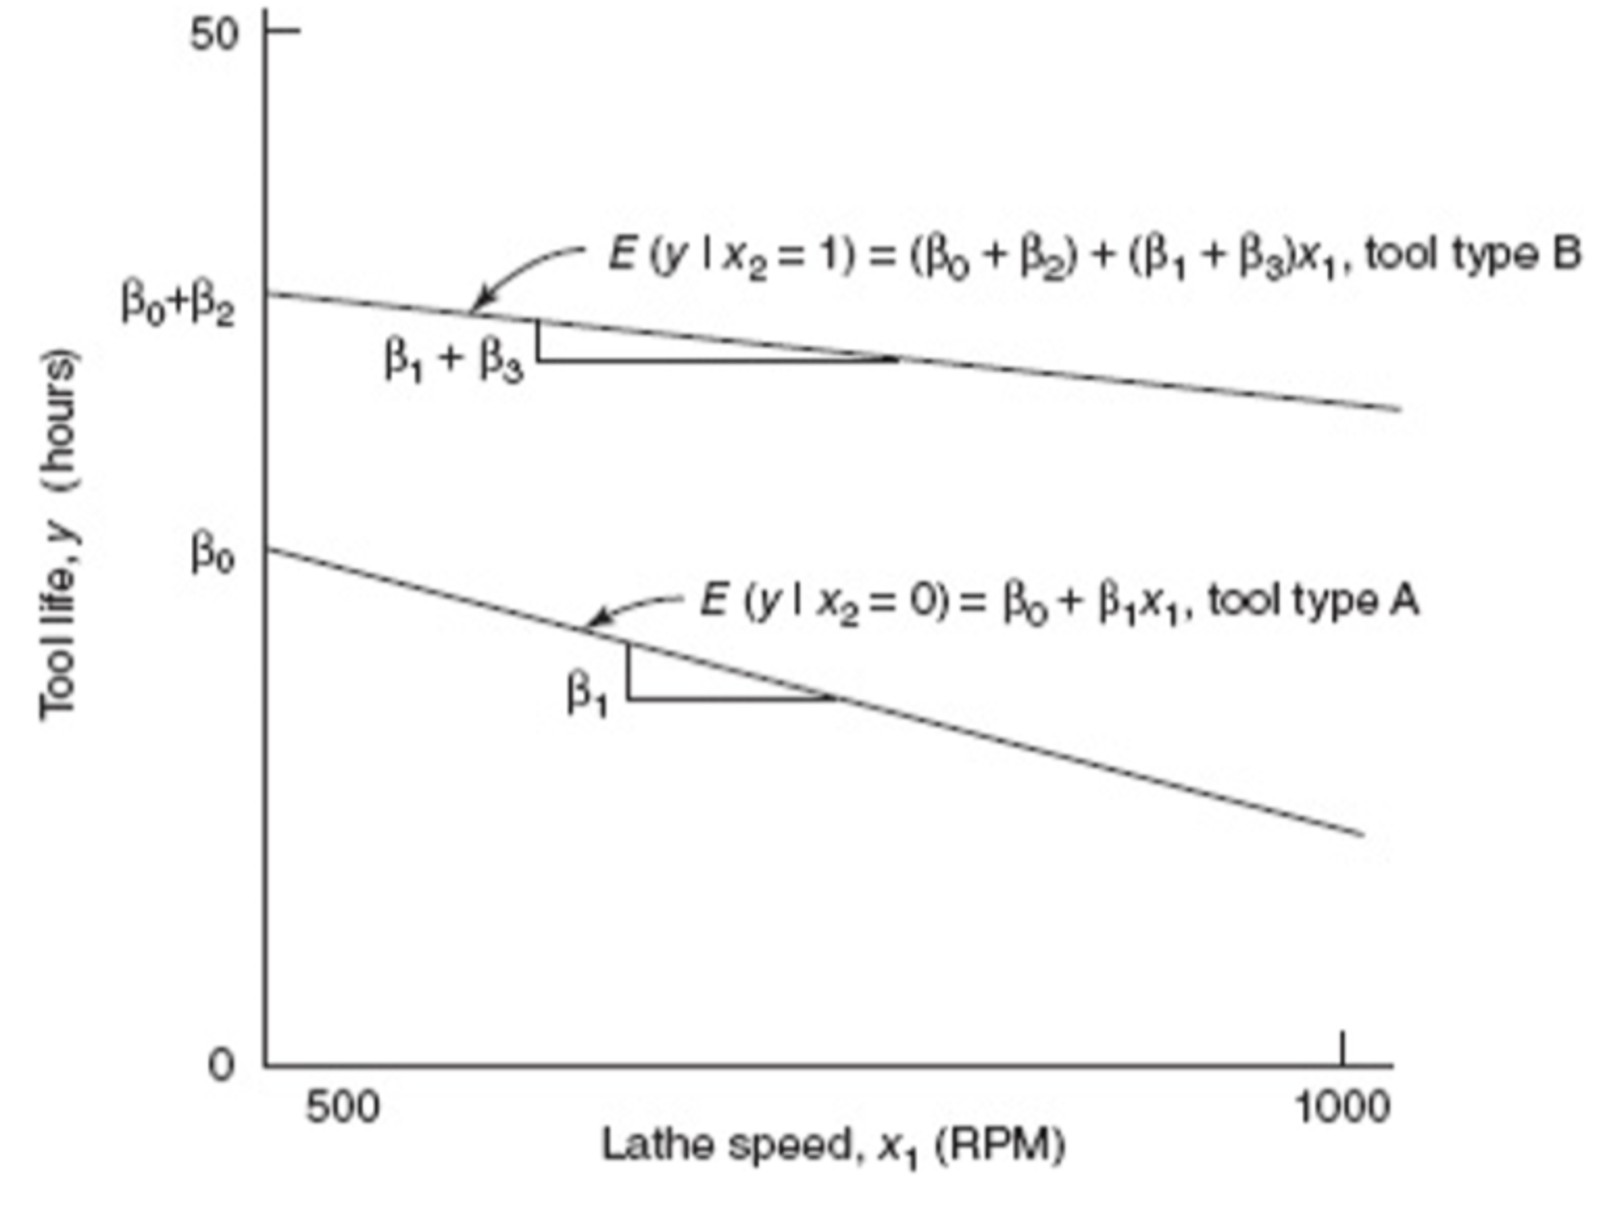
\includegraphics[width=\linewidth]{figures/interaction_term}
            To test if diff types are identical:\\
            $H_0:\beta_2 = \beta_3 = 0$ vs $H_1:\beta_2$ and/or $\beta_3 \neq 0$\\
            Note: we should not include $x_1x_2$ if there is no $x_2, x_1$
    \subsection{Standardised Regression Coefficients}
        \subsubsection{Unit normal Scaling}

        \begin{align*}
            x_{ij}=\frac{x_{ij}-\bar x_j}{s_j}, i\in[1, n], j\in[1, k]
        \end{align*}
        $\bar x_j = (\sum_{i=1}^nx_{ij})/n, s_j^2=(\sum_{i=1}^n(x_{ij}-\bar x_j)^2)/(n-1)$\\
        Note: model using scaled response and scaled regressors does not have intercept

        \subsubsection{Unit Length Scaling}

        \begin{align*}
            w_{ij}=\frac{x_{ij}-\bar x_j}{\sqrt{S_{jj}}}, i\in[1, n], j\in[1, k]
        \end{align*}
        $S_{jj} = \sum_{i=1}^n(x_{ij}-\bar x_j)^2=(n-1)s_j^2$\\
                Note: each new regressor $w_j$ has mean $\bar w_j = 0$ and length $\sqrt{\sum_{i=1}^n(w_{ij}-\bar w_j)^2}=1$\\
                The resultant $\bold{W^TW}$ matrix is a correlation matrix where $r_{lj}$ is simple correlation between $x_l, x_j$, $l, j = 1, \cdots, k, l\neq j$



	\subsection{Other topics}

		\subsubsection{Regression Through the Origin}
			$y = \beta_1x + \epsilon$, only appropriate when origin $(0,0)$ has meaning\\
			$\min S(\beta_1) = \sum_{i=1}^n(y_i-\beta_1x_i)^2$\\
			$\hat\beta_1 = {\sum_{i=1}^ny_ix_i}/{\sum_{i=1}^nx_i^2}$\\
			$\hat\sigma^2 = MS_{Res} = {\sum_{i=1}^n(y_i-\hat y_i)^2}/{n-1}$\\
			$=\left(\sum_{i=1}^ny_i^2-\hat\beta_1\sum_{i=1}^ny_ix_i\right)/(n-1)$

		\subsubsection{Estimation by Maximum Likelihood}
			Only when the response (or error) distribution is known\\
			i.e. $\epsilon \sim N(0, \sigma^2) \Rightarrow y_i \sim N(\beta_0 + \beta_1x_i, \sigma^2)$\\
			$\max L(y_i, x_i, \beta_0, \beta_1, \sigma^2) = \prod_{i=1}^n(2\pi\sigma^2)^{-1/2}exp\left[-\frac{1}{2\sigma^2}(y_i-\beta_0-\beta_1x_i)^2\right]$\\
			$=(2\pi\sigma^2)^{-n/2}exp\left[-\frac{1}{2\sigma^2}(y_i-\beta_0-\beta_1x_i)^2\right]$\\
			$\Leftrightarrow \max \log L = -\frac{n}{2}\log(2\pi)-\frac{n}{2}\log\sigma^2-\frac{1}{2\sigma^2}\sum_{i=1}^n(y_i-\beta_0-\beta_1x_i)^2$

			$\hat\beta_0=\bar y - \hat\beta_1\bar x$\\
			$\hat\beta_1 = {\sum_{i=1}^ny_i(x_i-\bar x)}/{\sum_{i=1}^n(x_i-\bar x)^2}$\\
			$\hat\sigma^2 = {\sum_{i=1}^n(y_i-\hat\beta_0-\hat\beta_1x_i)^2}/{n}=[(n-2)/n]\hat\sigma^2_{OLS}$, biased

    \section{Model Adequacy Checking}
    Model assumption:
        \begin{itemize}
            \item Linearity assumption $\bold{Y}=\bold{\beta X}$
            \item Normality assumption $\epsilon_i\sim N$
            \item $E(\epsilon)=0$
            \item Homogeneity assumption $Var(\epsilon)=\sigma^2$
            \item Independent error assumption $Cov(\epsilon_i, \epsilon_j)=0$
        \end{itemize}

        \subsection{Graphical Methods before model fitting}
        \begin{itemize}
            \item One-dimensional graphs
                \subitem Histogram, Stem-and-leaf-display, Dot plot, Box plot (for outlier detection)
                \subitem Check for: 1) distribution (symmetric or skewed) to determine if transformation is required 2) outliers
            \item Two-dimensional graphs
                \subitem pairwise plots (e.g. scatter plots)
                \subitem Check for: 1) Multicollinearity 2) Linear relationship $y\sim x$
            \item Rotating plots
            \item Dynamic graphs
        \end{itemize}

        \subsection{Residual Analysis}
        Diagnostic methods primarily based on studying model residuals ($e_i=y_i-\hat y_i)$
        \begin{align*}
            E(e_i) &= 0\\
            Var(\bar e) &= \frac{\sum_{i=1}^n(e_i-\bar e)^2}{n-p} = \frac{\sum_{i=1}^n e_i^2}{n-p} = \frac{SS_{Res}}{n-p} = MS_{Res}
        \end{align*}
        The residuals are not independent. However, when $p << n$ the nonindependence has little effect

        \subsubsection{Hat Matrix}
        \begin{align*}
        \bold{H}&\bold{=X(X'X)^{-1}X'}\\
        \bold{\hat y} &= \bold{Hy}\\
        \hat y_i &= h_{i1}y_1 + \cdots + h_{in}y_n\\
        \bold{e} &= \bold{(I-H)y}
        \end{align*}
        \begin{tabulary}{\linewidth}{l@{ := }L}
            $\hat y_i$ & weighted sum of all given observation\\
            $h_{ii}$ & leverage value for $i$th observation\\
                     & weight given to $y_i$ in determining the $i$th fitted values $\hat y_i$\\
            $\bold{H}$ & is symmetric and idempotent ($\bold{HH=H}$)\\
            $\bold{I-H}$ & is symmetric and idempotent
        \end{tabulary}


        \subsubsection{Variance of Residuals}

        \begin{align*}
            \bold{e} &= \bold{(I-H)(X\beta+\epsilon)}\\
                     &= \bold{(I-H)\epsilon}\\
            Var(\bold{\epsilon}) &= \sigma^2\bold{I}\\
            Var(\bold{e}) &= \bold{(I-H)}Var(\bold{\epsilon})\bold{(I-H)'} = \sigma^2\bold{(I-H)}\\
            Var(e_i) &= \sigma^2(1-h_{ii})\\
        Cov(e_i, e_j) &=-\sigma^2h_{ij}
        \end{align*}

        \subsubsection{Standardized Residual}
        \begin{align*}
            &\frac{e_i}{\sigma\sqrt{(1-h_{ii})}}\\
            \hat\sigma^2_{(i)} &= \frac{SS_{Res(i)}}{n-k-2} = \frac{SS_{Res(i)}}{n-p-1}
        \end{align*}
        Estimate $\sigma^2$: $MS_{Res}$ or $\hat\sigma^2_{(i)}$, both unbiased estimator of $\sigma^2$\\
        $SS_{Res(i)}$ := sum of squared residual when fit model with $(n-1)$ obs without $i$th obs

        \subsubsection{Studentized Residuals}
        Internally studentized residuals
        \begin{align*}
            r_i = \frac{e_i}{\sqrt{MS_{Res}}\sqrt{(1-h_{ii})}}
        \end{align*}
    \begin{lstlisting}{R}
rstandard(model)
    \end{lstlisting}
    Externally studentized residuals
    \begin{align*}
        r^*_i &= \frac{e_i}{\hat\sigma_{(i)}\sqrt{(1-h_{ii})}}\\
        r^*_i &= r_i \sqrt{\frac{n-p-1}{n-p-r_i^2}}
    \end{align*}
    Since both internal and external studentized residuals are monotone transformation of another, either is fine

        \subsubsection{Residual plots}
        Normal Probability Plot (QQ plot)
        \begin{itemize}
            \item Plot ordered S.R (x-axis) vs cumulative probability or normal scores (y-axis)
                \subitem Expect: normally distributed residuals, nearly straight line with an intercept of 0 and slope 1
                \subitem Note: common defect is due to large residuals arise from outliers
        \end{itemize}
        Scatter plot of S.R. vs fitted values
        \begin{itemize}
            \item Plot residuals vs fitted values
                \subitem Expect: random scatter plot
                \subitem Note: observe for potential patterns, such as non-constant variance, nonlinearity
        \end{itemize}
        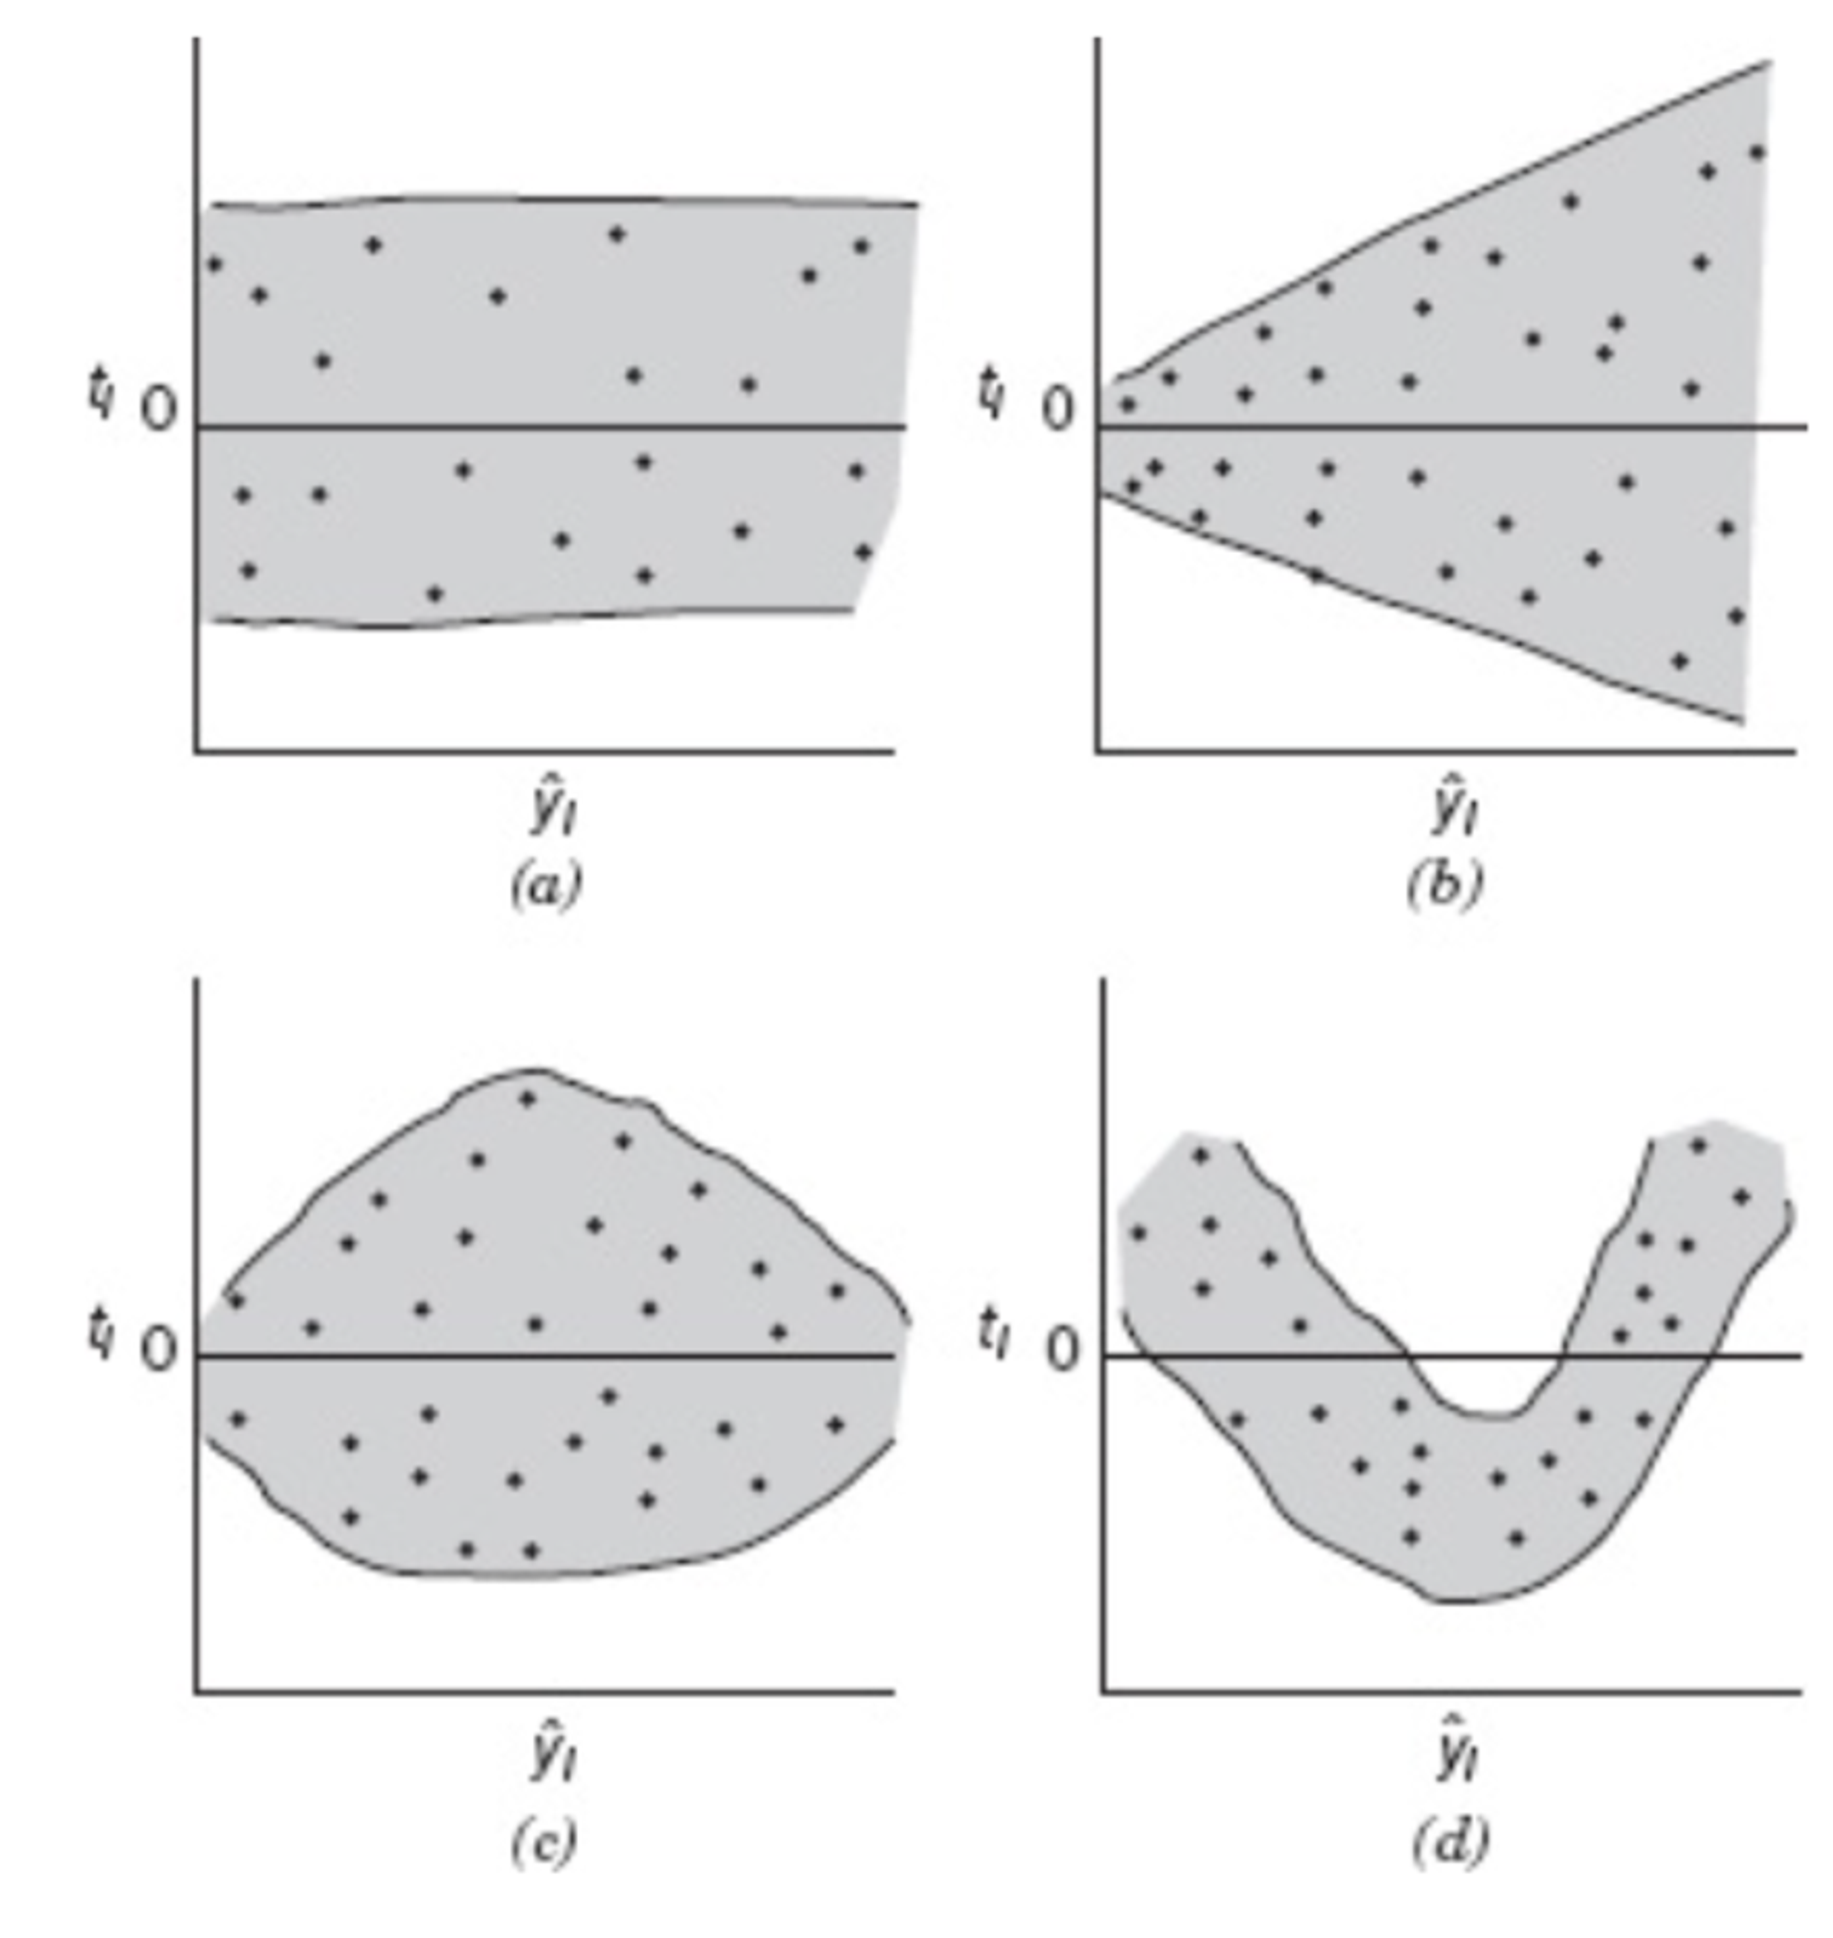
\includegraphics[width=\linewidth]{figures/residual_plot}
        \begin{itemize}
            \item[a] ideal
            \item[b] non constant variance (heterogeneity)
            \item[c] variance follow binomial distribution
            \item[d] non linear relationship
        \end{itemize}
        Scatter plots of S.R. vs each predictor
        \begin{itemize}
            \item Plot S.R. with each regressors
                \subitem Except: randomly scattered plot
                \subitem Note: transformation might be needed for the regressors
        \end{itemize}
        Plot of Residuals in Time Sequence
        \begin{itemize}
            \item Plot residuals against time order
            \subitem Expect: randomly scatter plot
            \subitem Note: if not random, variance might be changing with time then linear or quadratic terms in time should be added to the model
        \item Autocorrection (errors are related to each other) is serious violation of basic regression assumptions
        \end{itemize}

        \subsubsection{Comments on Residual plots}
        \begin{itemize}
            \item Strong indication of linear relationship between variables
            \item Normal probability plot indicates a deviation from normality assumption, it also shows potential outliers
            \item plot of residuals vs fitted values has large residuals, suggesting outliers
            \item Scatter plot between regressors show linear relationship between them, a deeper investigation about data is needed. There might be ommitted variable bias (factors that linked to both regressors such as location), extra variables should be added to fix this
        \end{itemize}

        \subsection{Detection and Treatment of Outliers}
        Outlier:
        \begin{itemize}
            \item extreme observation, one that is considerably different from the majority of data
            \item Residuals $>> 3$ sd from mean indicate potential $y$ space  outliers
            \item 1) Examine Residual plots against fitted values
            \item 2) QQ-plot
            \item "bad" values: result of unusual but explainable events, can be deleted and corrected
                \subitem e.g. faulty measurement or analysis, incorrect recording data, failure of measuring instrument
            \item "normal" values: unusual but perfectly pausible observation
                \subitem should be kept since deleting will provide false sense of precision in estimation/prediction
        \end{itemize}
        Observe (compare with and without outliers):
        \begin{itemize}
            \item Changes in goodness of fit ($R^2$, $MS_{Res}$)
            \item Effect on model (magnitude and sign of $\beta$)
        \end{itemize}

        \subsection{Lack of Fit of the Regression Model}
        Formal test for Lack of fit (only for simple model)
        \begin{align*}
            y_{ij} - \hat y_i &= (y_{ij} - \bar y_i) + (\bar y_i - \hat y_i)\\
            \sum_{i=1}^m \sum_{j=1}^{n_i}(y_{ij} - \hat y_i)^2 &=
            \sum_{i=1}^m\sum_{j=1}^{n_i}(y_{ij} - \bar y_i)^2 +
            \sum_{i=1}^m {n_i} (\bar y_i-\hat y_i)^2\\
            SS_{Res} &= SS_{PE} + SS_{LOF}\\
            F_0 &= \frac{SS_{LOF}/(m-2)}{SS_{PE}/(n-m)} = \frac{MS_{LOF}}{MS_{PE}}\\
                &\sim F_{m-2, n-m}
        \end{align*}
        Assumption: normality, independence and constant variance. Test only the first order relationship
        \begin{align*}
            H_0: \beta_1 \neq 0
        \end{align*}
        \begin{tabulary}{\linewidth}{l @{ := }L}
            $m$ & num of levels ($x$ into $m$ groups)\\
            $n$ & $\sum_{i=1}^m n_i$ total observation\\
            $ij$ residual & $y_{ij}-\hat y_i$\\
            $SS_{PE}$ & sum of squaress due to pure error\\
            $SS_{LOF}$ & sum of squares due to lack of fit
        \end{tabulary}

        \subsection{Leverage and Influence}
        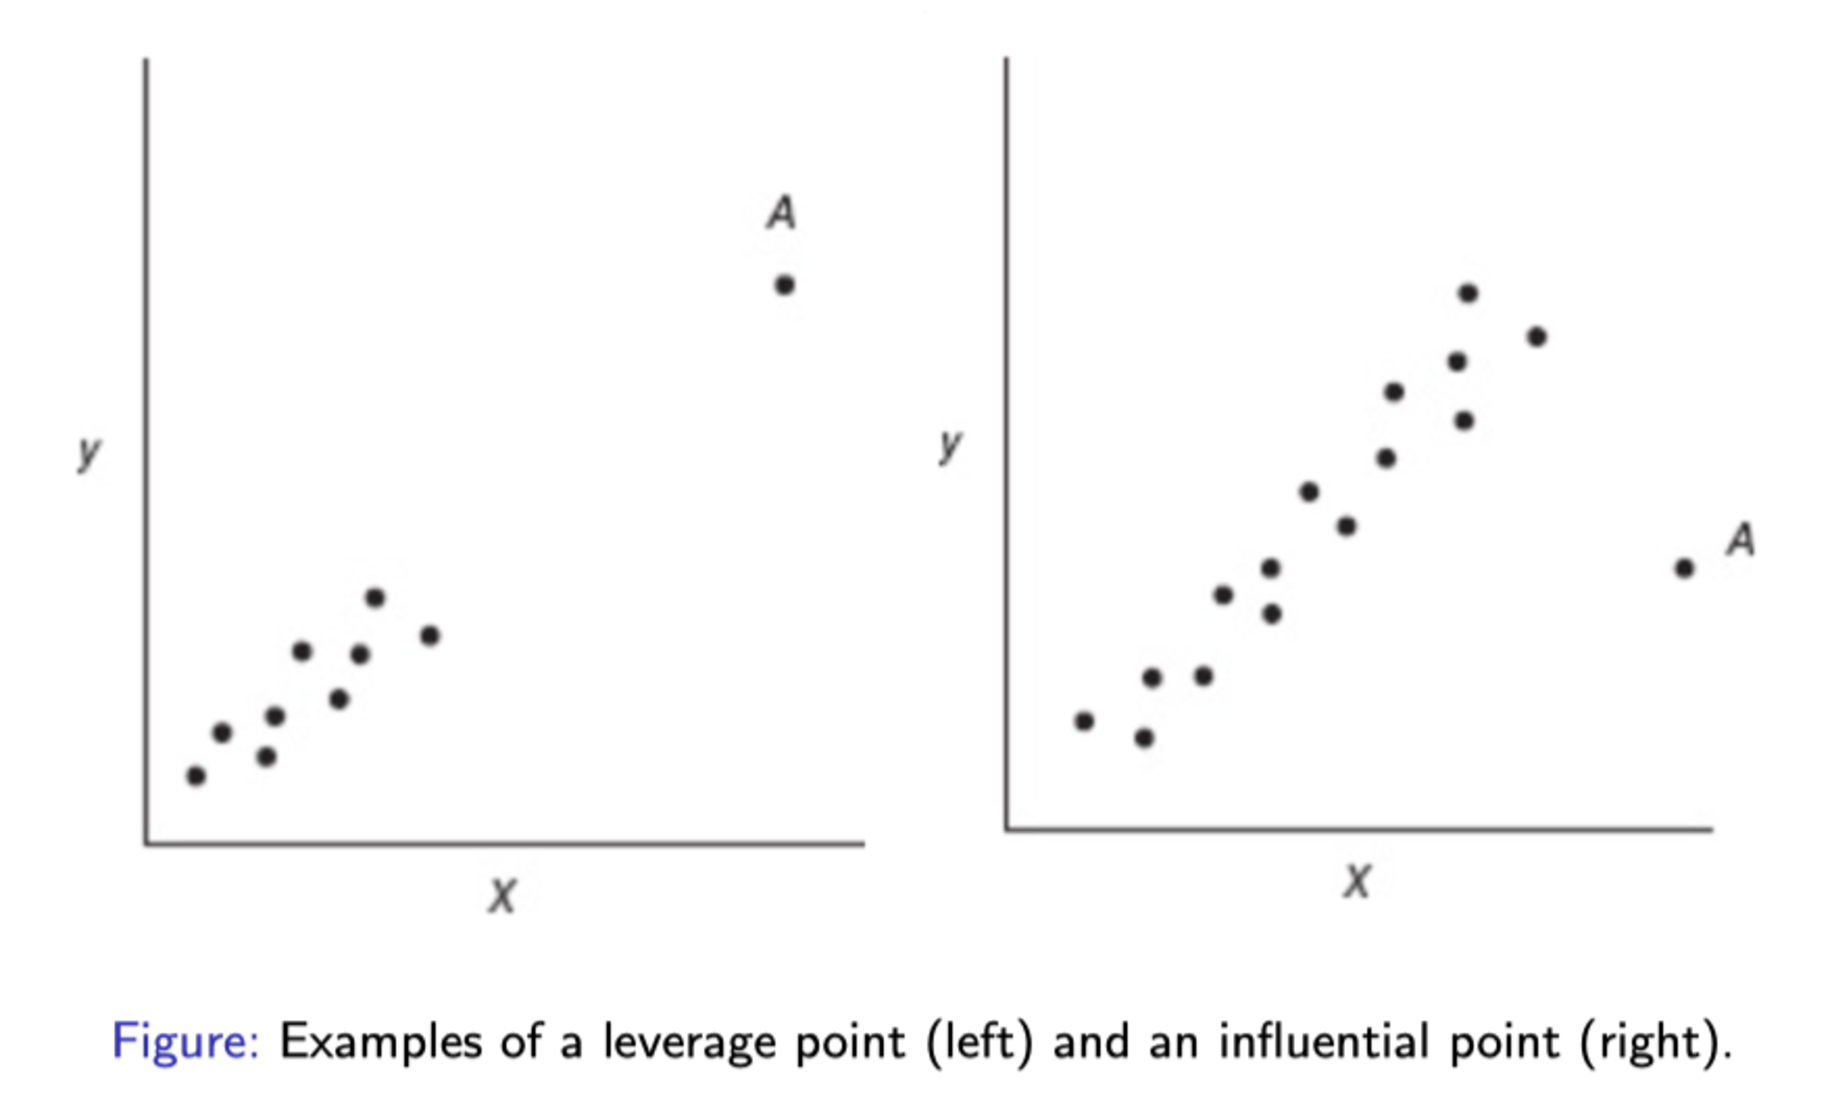
\includegraphics[width=\linewidth]{figures/leverage_influence}

        \subsubsection{Diagnostics for Leverage}
        \begin{align*}
            h_{ii} &= x_i(\bold{X'X})^{-1}x_i'
        \end{align*}
        \begin{itemize}
            \item standardised distance of $i$th observation from the center of the $x$ space
            \item the amount of leverage exerted by $j$th observation $y_j$ on the fitted value $\hat y_i$.
            \item Large $h_{ii}$ indicate potential influential
            \item Not all leverage points are influential points. Should consider $h_{ii}$ with standardized residuals. Large for both are likely to be influential
            \item since $\sum h_{ii}=rank(\bold{H})=rank(\bold{X})=p$, average size of $h_{ii}$ is $\bar h = p/n$
            \item $h_{ii} > 2p/n$ is consider leverage point (for small sample where $2p/n>1$ then this cutoff doesn't apply)
\end{itemize}
    \begin{lstlisting}[language=R]
# include beta0
x <- cbind(c(rep(1, n), x1, x2)
# hat matrix
hat <- x%*%solve(t(x)%*%x)%*%t(x)
which(diag(hat)>(2p/n))
    \end{lstlisting}

        \subsubsection{Cook's Distance}
        Measure of influence\\
        $\beta_{(i)}:=$ beta without the $i$th data\\
        Usual choice of $\bold{M}=\bold{X'X}, c=pMS_{res}$
        \begin{align*}
            D_i = (\bold{M}, c) = \frac{(\hat\beta_{(i)}-\hat\beta)'\bold{M}(\hat\beta_{(i)}-\hat\beta)}{c}, i\in[1,n]
        \end{align*}
        Points with large $D_i$ have considerable influence on the least square estimate $\hat\beta$
        \begin{align*}
            D_i = \frac{r^2_i}{p}\frac{h_{ii}}{1-h_{ii}} \sim F_{p, n-p}(\alpha)
        \end{align*}
        Deleting point $i$ would move the estimate of $\bold{\beta}$ to approximately the edge of a $F^{-1}_{p, n-p}(D_i)$ confidence region.
    \begin{lstlisting}[language=R]
cook.distance(model)
    \end{lstlisting}

        \subsubsection{DFFITS, DFBETAS}
        \begin{itemize}
            \item Statistic that indicate how much $\hat\beta_j$ changes in standard deviation if $i$ was deleted
            \item Number of standard deviation that the fitted value $\hat y_i$ changes if observation $i$ was removed
        \end{itemize}

    \section{To Correct Model Inadequacies}

        \subsection{Transformation to Linearize the model}
    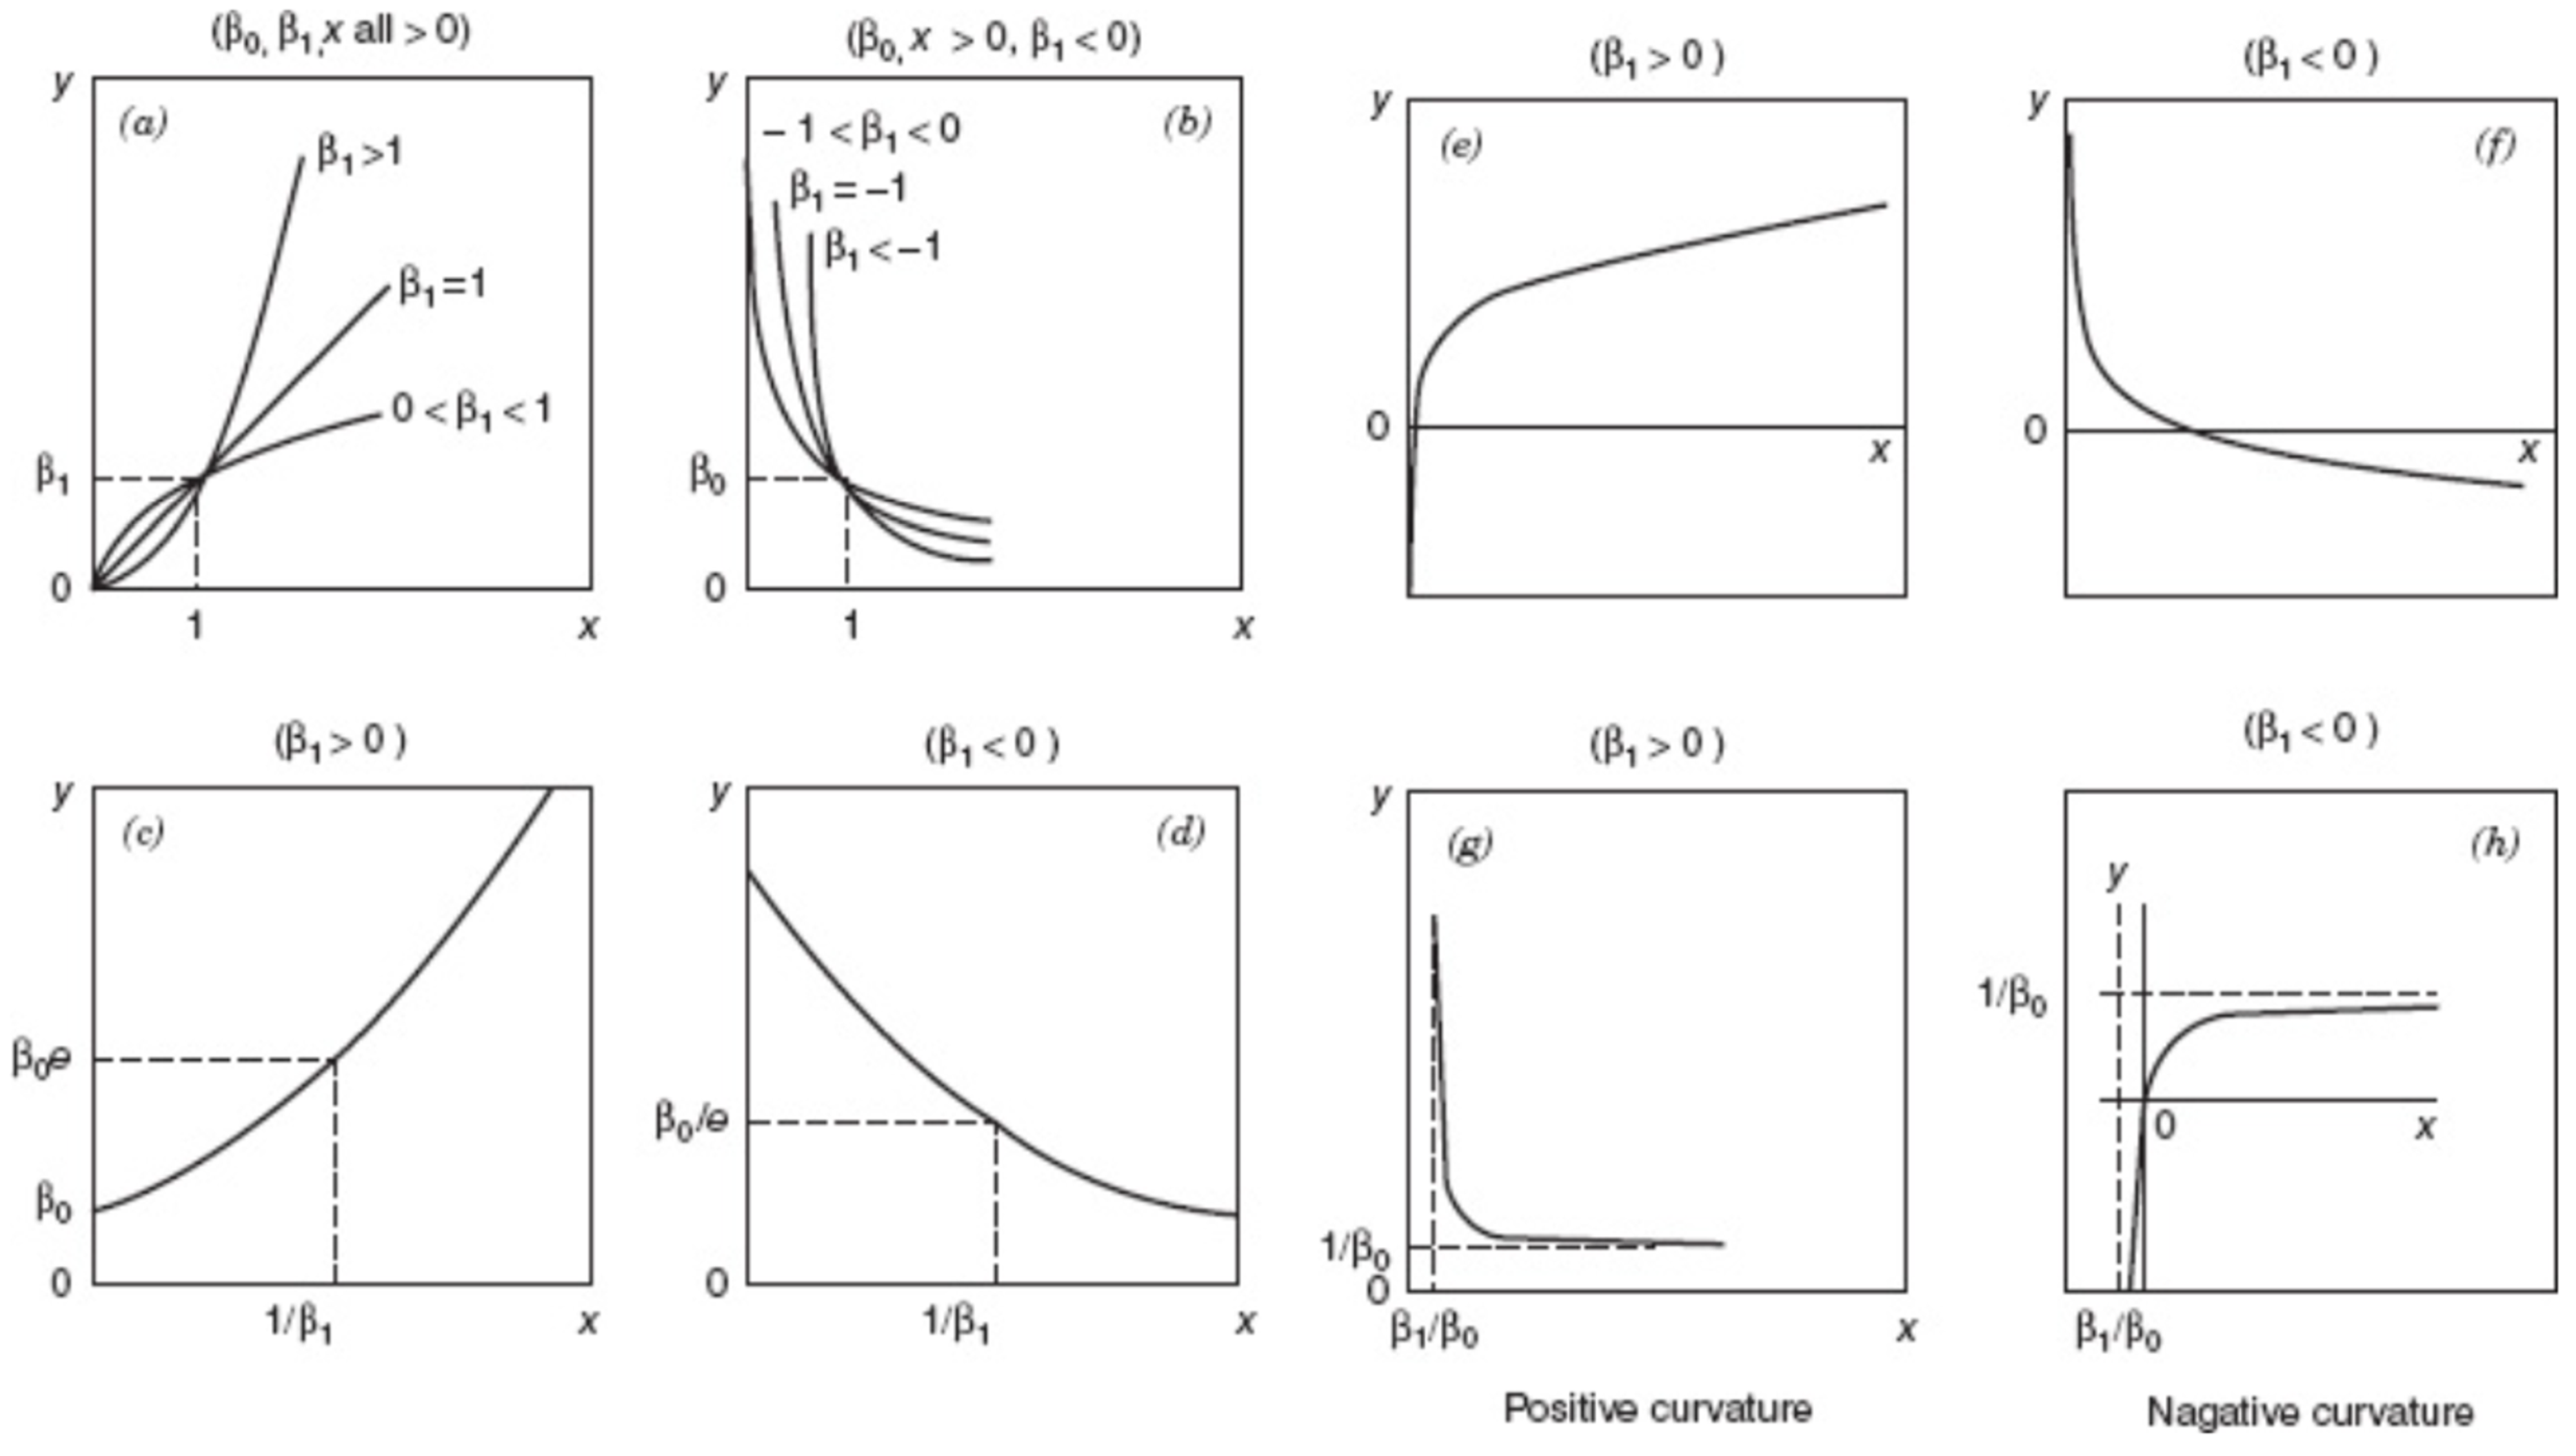
\includegraphics[width=\linewidth]{figures/linearizable_functions.pdf}
    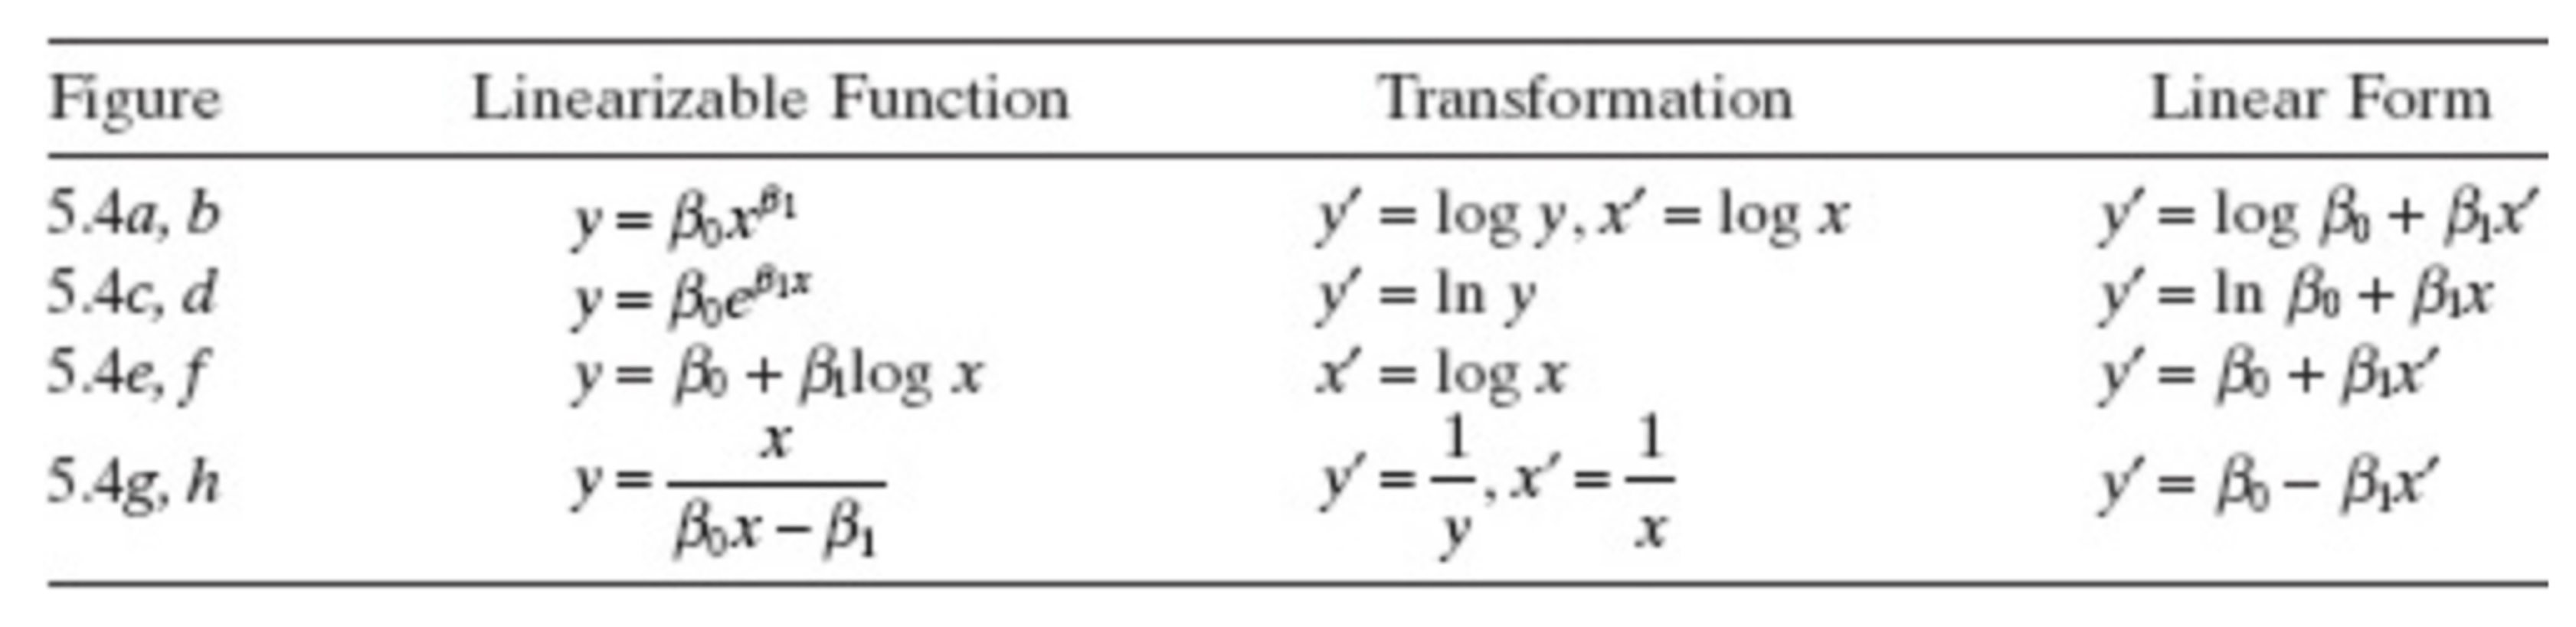
\includegraphics[width=\linewidth]{figures/corresponding_linear_forms.pdf}
	\begin{lstlisting}[language=R]
model <- lm(y~I(x^2)+I(1/X))
    \end{lstlisting}

        \subsection{Analytical Methods for Selecting a Transformation}

        \subsubsection{Transformation on $y$: Box-Cox Method}
        Power transformation $y^\lambda$ using maximum likelihood\\
        Estimate $\bold{\beta}, \lambda$
        \begin{align*}
            y^{(\lambda)} &= \begin{cases}
                \frac{y^\lambda -1}{\lambda y \dot{y} y^{\lambda-1}}, &\lambda \neq 0\\
                \dot{y} log(y), &\lambda =0
            \end{cases}\\
                \dot{y} &= exp[\frac{1}{n}\sum_{i=1}^nlog(y_i)]\\
                \bold{y}^{(\lambda)} &= \bold{X\beta+\epsilon}
        \end{align*}
        Transform $y=y^{(\lambda)}$ if $\lambda \neq 0$ else $log(y)$
    \begin{lstlisting}[language=R]
library(MASS)
boxcox(model, lambda=seq(-2, 2, 0.5),
        optimize=TRUE, plotit=TRUE)
    \end{lstlisting}

        \subsubsection{Transformation on $X$: Box and Tidwell}
        Estimate $\beta_0, \beta_1, \alpha$
        \begin{align*}
            \xi &= \begin{cases}
                x^{\alpha}, &\alpha\neq0\\
                log(x), &\alpha=0
            \end{cases}
        \end{align*}
        To estimate $\alpha$
        \begin{enumerate}
            \item Initial a model by least square method
                \subitem $\hat y = \hat \beta_0 + \hat \beta_1 x$
            \item fit a new model adding $w=xlog(x)$
                \subitem $\hat y = \hat\beta_0'+\hat\beta_1'x+\hat\gamma w$
            \item then take
                \subitem $\alpha_1=(\hat\gamma/\hat\beta_1)+1$
        \end{enumerate}
        Repeat procedure (1-3) with $x'=x^{\alpha_1}$\\
        Procedure converge rapidly, often first stage result $\alpha$ is a satisfactory estimate of $\alpha$

        \subsection{Generalized and Weighted Least Squares}

        \subsubsection{Weighted Least Squares}
        Linear regression models with nonconstant variance.\\
        Deviation between $y_i, \hat y_i$ is multiplied by a weight $w_i\propto1/Var(y_i)$\\
        WLS estimators are unbiased\\
        $MS_{(w)RES}$ is unbiased estimator of $\sigma^2$\\
        \begin{align*}
            S(\beta_0, \beta_1) &= \sum_{i=1}^n w_i(y_i-\beta_0-\beta_1x_i)^2\\
            w_i &= \frac{1}{\sigma_i^2}\\
            w_i = w_j &\Leftrightarrow \sigma_i = \sigma_j\\
            \hat\beta_0 &= \bar y_w - \hat\beta_1 \bar x_w\\
            \hat\beta_1 &= \frac{\sum_{i=1}^n w_i(x_i-\bar y_w)(y_i-\bar x_w)}{\sum_{i=1}^n w_i(x_i-\bar x_w)^2}\\
            \bar x_w = \frac{\sum_{i=1}^n w_ix_i}{\sum_{i=1}^n w_i}~~~ &
            \bar y_w = \frac{\sum_{i=1}^n w_iy_i}{\sum_{i=1}^n w_i}
        \end{align*}
        Benefits
        \begin{itemize}
            \item In transformed model, coefficient estimates are hard to interpret. Interpretation for WLS remain the same
            \item WLS can remove an observation by setting weight = 0
            \item WLS also can weight down outlier and influential point
        \end{itemize}

        \subsubsection{Generalized Least Squares}
        \begin{align*}
            \bold{y} &= \bold{X\beta+\epsilon}\\
            E(\bold{\epsilon})=0~~&~~Var(\bold{\epsilon}) = \sigma^2\bold{V}\\
        \end{align*}
        \begin{itemize}
            \item OLS: $\bold{V=I}$
            \item WLS: $\bold{V}$ is diagonal, $\bold{y}$ are uncorrelated but have unequal variances
            \item if off-diagonal $\bold{V}$ are nonzero, then observations are correlated
        \end{itemize}
        Least squares normal equation
        \begin{align*}
            \bold{(X'V^{-1}X)}\hat\beta &= \bold{X'V^{-1}y}\\
            \bold{\hat\beta} &= \bold{(X'V^{-1}X)^{-1}X'V^{-1}y}
        \end{align*}
        $\bold{\hat\beta}$ is the generalized least squares estimate of $\bold{\beta}$

    \section{Multicollinearity}
    Multicollinearity occur when regressors are not orthogonal to each other\\
    Let $X_j$ be the $j$th column of the matrix $X$, if
    \begin{align*}
        \sum_{j=1}^k t_j\bold{X_j}=0
    \end{align*}
    where $t_j$ are not all zero is approximately true then $\bold{X'X}^{-1}$ does not exist

        \subsection{Sources of Multicollinearity}
        \begin{itemize}
            \item Data collection method
                \subitem occur when only subsample of the entire sample space has been selected
                \subitem if positive correlation is strong enough, multicollinearity problem will occur
            \item Constraints on the model or in the population
                \subitem physical constraint regardless of collection method
            \item Model specification
                \subitem adding polynomial term of regressors
            \item Overdefined model
                \subitem fit more regressors than observations
                \subitem solve by: 1. using lesser regressors 2. do preliminary studies using subset of regressors 3. use principal components
        \end{itemize}

        \subsection{Effects of Multicollinearity}

        \subsubsection{Poor Coefficient Estimate}
        $\bold{C:=(X'X)^{-1}}$ with only $k$ regressors\\
        $L_1^2:=$ squared distance between $\hat\beta$ and $\beta$
        \begin{align*}
            L_1^2 &= \bold{(\hat\beta-\beta)'(\hat\beta-\beta)}\\
        E(L_1^2) &= E[\bold{(\hat\beta-\beta)'(\hat\beta-\beta)}] = \sum_{j=1}^k E(\hat\beta_j-\beta_j)^2\\
		     &=\sum_{j=1}^k Var(\hat\beta_j) = \sigma^2 Tr(X'X)^{-1}\\
            E(L_1^2) &= \sigma^2 \sum_{j=1}^k \frac{1}{\lambda_j}
        \end{align*}
        $\lambda_j:=$ $j$th eigenvalues of $\bold{X'X}$\\
        Trace of matrix is sum of the eigenvalues of matrix\\
        When multicollinearity presents, at least one of $\lambda_j$ is large.
        Therefore, distance from $\bold{\hat\beta}$ to $\bold{\beta}$ is large.

        \subsubsection{Large Variances and Covariances}
        if $\bold{X}$ is unit length scaled matrix
        \begin{align*}
            Cor(\bold{X}) &= \bold{X'X}\\
            [Cor(\bold{X})]^{-1}=\bold{C} &= \frac{1}{1-R^2_j}\\
            Var(\hat\beta_j) &= \sigma^2C_{jj}
        \end{align*}
        $R^2_j:=$ multiple coefficient of determination from the regression of $x_j$ on the remaining $k-1$ regressor variables\\
        If multicollinearity presents, one of $R^2_j$ will be large and $Var(\beta_j)$ will be large

        \subsection{Multicollinearity Diagnostics}

        \subsubsection{Examination of the Correlation Matrix}
        Unit scaled $\bold{X}$ without intercept
        \begin{align*}
            r_{ij} \text{ of } \bold{X'X} = cor(\bold{X})
        \end{align*}
        if $|r_{ij}|$ is close to 1, there might be multicollinearity.

        \subsubsection{Variance Inflation Factors}
        Since $Var(\beta_j)=\sigma^2C_{jj}$. $C_jj$ increase with VIF. \\
        VIF is the factor by which variance increase due to near-linear dependence among the regressors
        \begin{align*}
            VIF_j = \frac{1}{1-R_j^2}
        \end{align*}
        If $VIF_j > 5$, associated regression coefficient are poorly estimated due to multicollinearity
        \begin{lstlisting}[language=R]
diag(solve(t(X)%*%X))
diag(solve(cor(X)))
            \end{lstlisting}

        \subsubsection{Eigensystem Analysis of $\bold{X'X}$}
        eigenvalues of $\bold{A}_{k\times k}$ are the $k$ roots of the equation $|\bold{A}-\lambda\bold{I}|=0$
            \begin{lstlisting}[language=R]
eigen(X)$values
            \end{lstlisting}
        small eigenvalues are indications of multicollinearity
        \begin{align*}
            \text{Kappa } k &= \frac{\lambda_{max}}{\lambda_{min}}\\
            k_j &= \frac{\lambda_{max}}{\lambda_j}
        \end{align*}
        \begin{itemize}
            \item $K < 100$: no serious problem
            \item $100<l<1000$: moderate to strong multicollinearity
            \item $k>1000$: strong multicollinearity
        \end{itemize}
        Eigensystem analysis can be used to identify the nature of the near-linear dependence in data (self-study)

        \subsection{Methods for Dealing with Multicollinearity}
        \begin{itemize}
            \item Collect more data
            \item Respecify the model
            \item Ridge Regression or Principal Component Regression
        \end{itemize}

        \subsubsection{Ridge Regression}
        $\bold{X'X}$ in correlation form
        \begin{align*}
            \bold{(X'X+\lambda\bold{I}})\bold{\hat\beta_R} &= \bold{X'y}\\
            \bold{\hat\beta_R} &= (\bold{X'X+}\lambda\bold{I)^{-1}X'y}\\
                               &=(\bold{X'X+}\lambda\bold{I)^{-1}X'X\hat\beta}\\
                               &=\bold{Z_\lambda\hat\beta}
        \end{align*}
        when $\lambda=0$, ridge is least squares estimate
        \begin{align*}
            MSE(\bold{\hat\beta_R}) &= Var(\bold{\hat\beta_R}) + (\text{bias in }\bold{\hat\beta_R})^2\\
                                    &=\sigma^2\sum_{j=1}^k\frac{\lambda_j}{(\lambda_j+\lambda)^2}+
                                    \lambda^2\bold{\beta'(X'X+}\lambda\bold{I})^{-2}\bold{\beta}
        \end{align*}
        $\lambda$ increase: Var decrease bias increase\\
    Hoerl and Kennard proved there exist a non-zero $\lambda$ s.t. MSE of $\hat\beta_R$ $<Var(\hat\beta)$ from OLS.
    provided $\bold{\hat\beta'\beta}$ is bounded
    \begin{align*}
        SS_{Res} &= \bold{(y-X\hat\beta_R)'(y-X\hat\beta_R)}\\
                 &=\bold{(y-X\hat\beta)(y-X\hat\beta)+(\hat\beta_R-\hat\beta)'X'X(\hat\beta_R-\hat\beta)}
    \end{align*}
    Term of LHS is $SS_{Res}$ for OLS $\hat\beta$\\
    Ridge estimates will not necessarily provide the best "fit" to the data.
    When $\lambda$ increase, $SS_{Res}$ of $\hat\beta_R$ increase and $R^2$decrease
            \begin{lstlisting}[language=R]
library(MASS)
lm.ridge(y~x, data=data, lambda=)
library(lmridge)
lmridge(y~x, data=data, K=)
summary(model) # only lmridge
            \end{lstlisting}

        \subsubsection{Ridge Trace}
        Objective: finding smallest possible $\lambda$ s.t. line is stable
        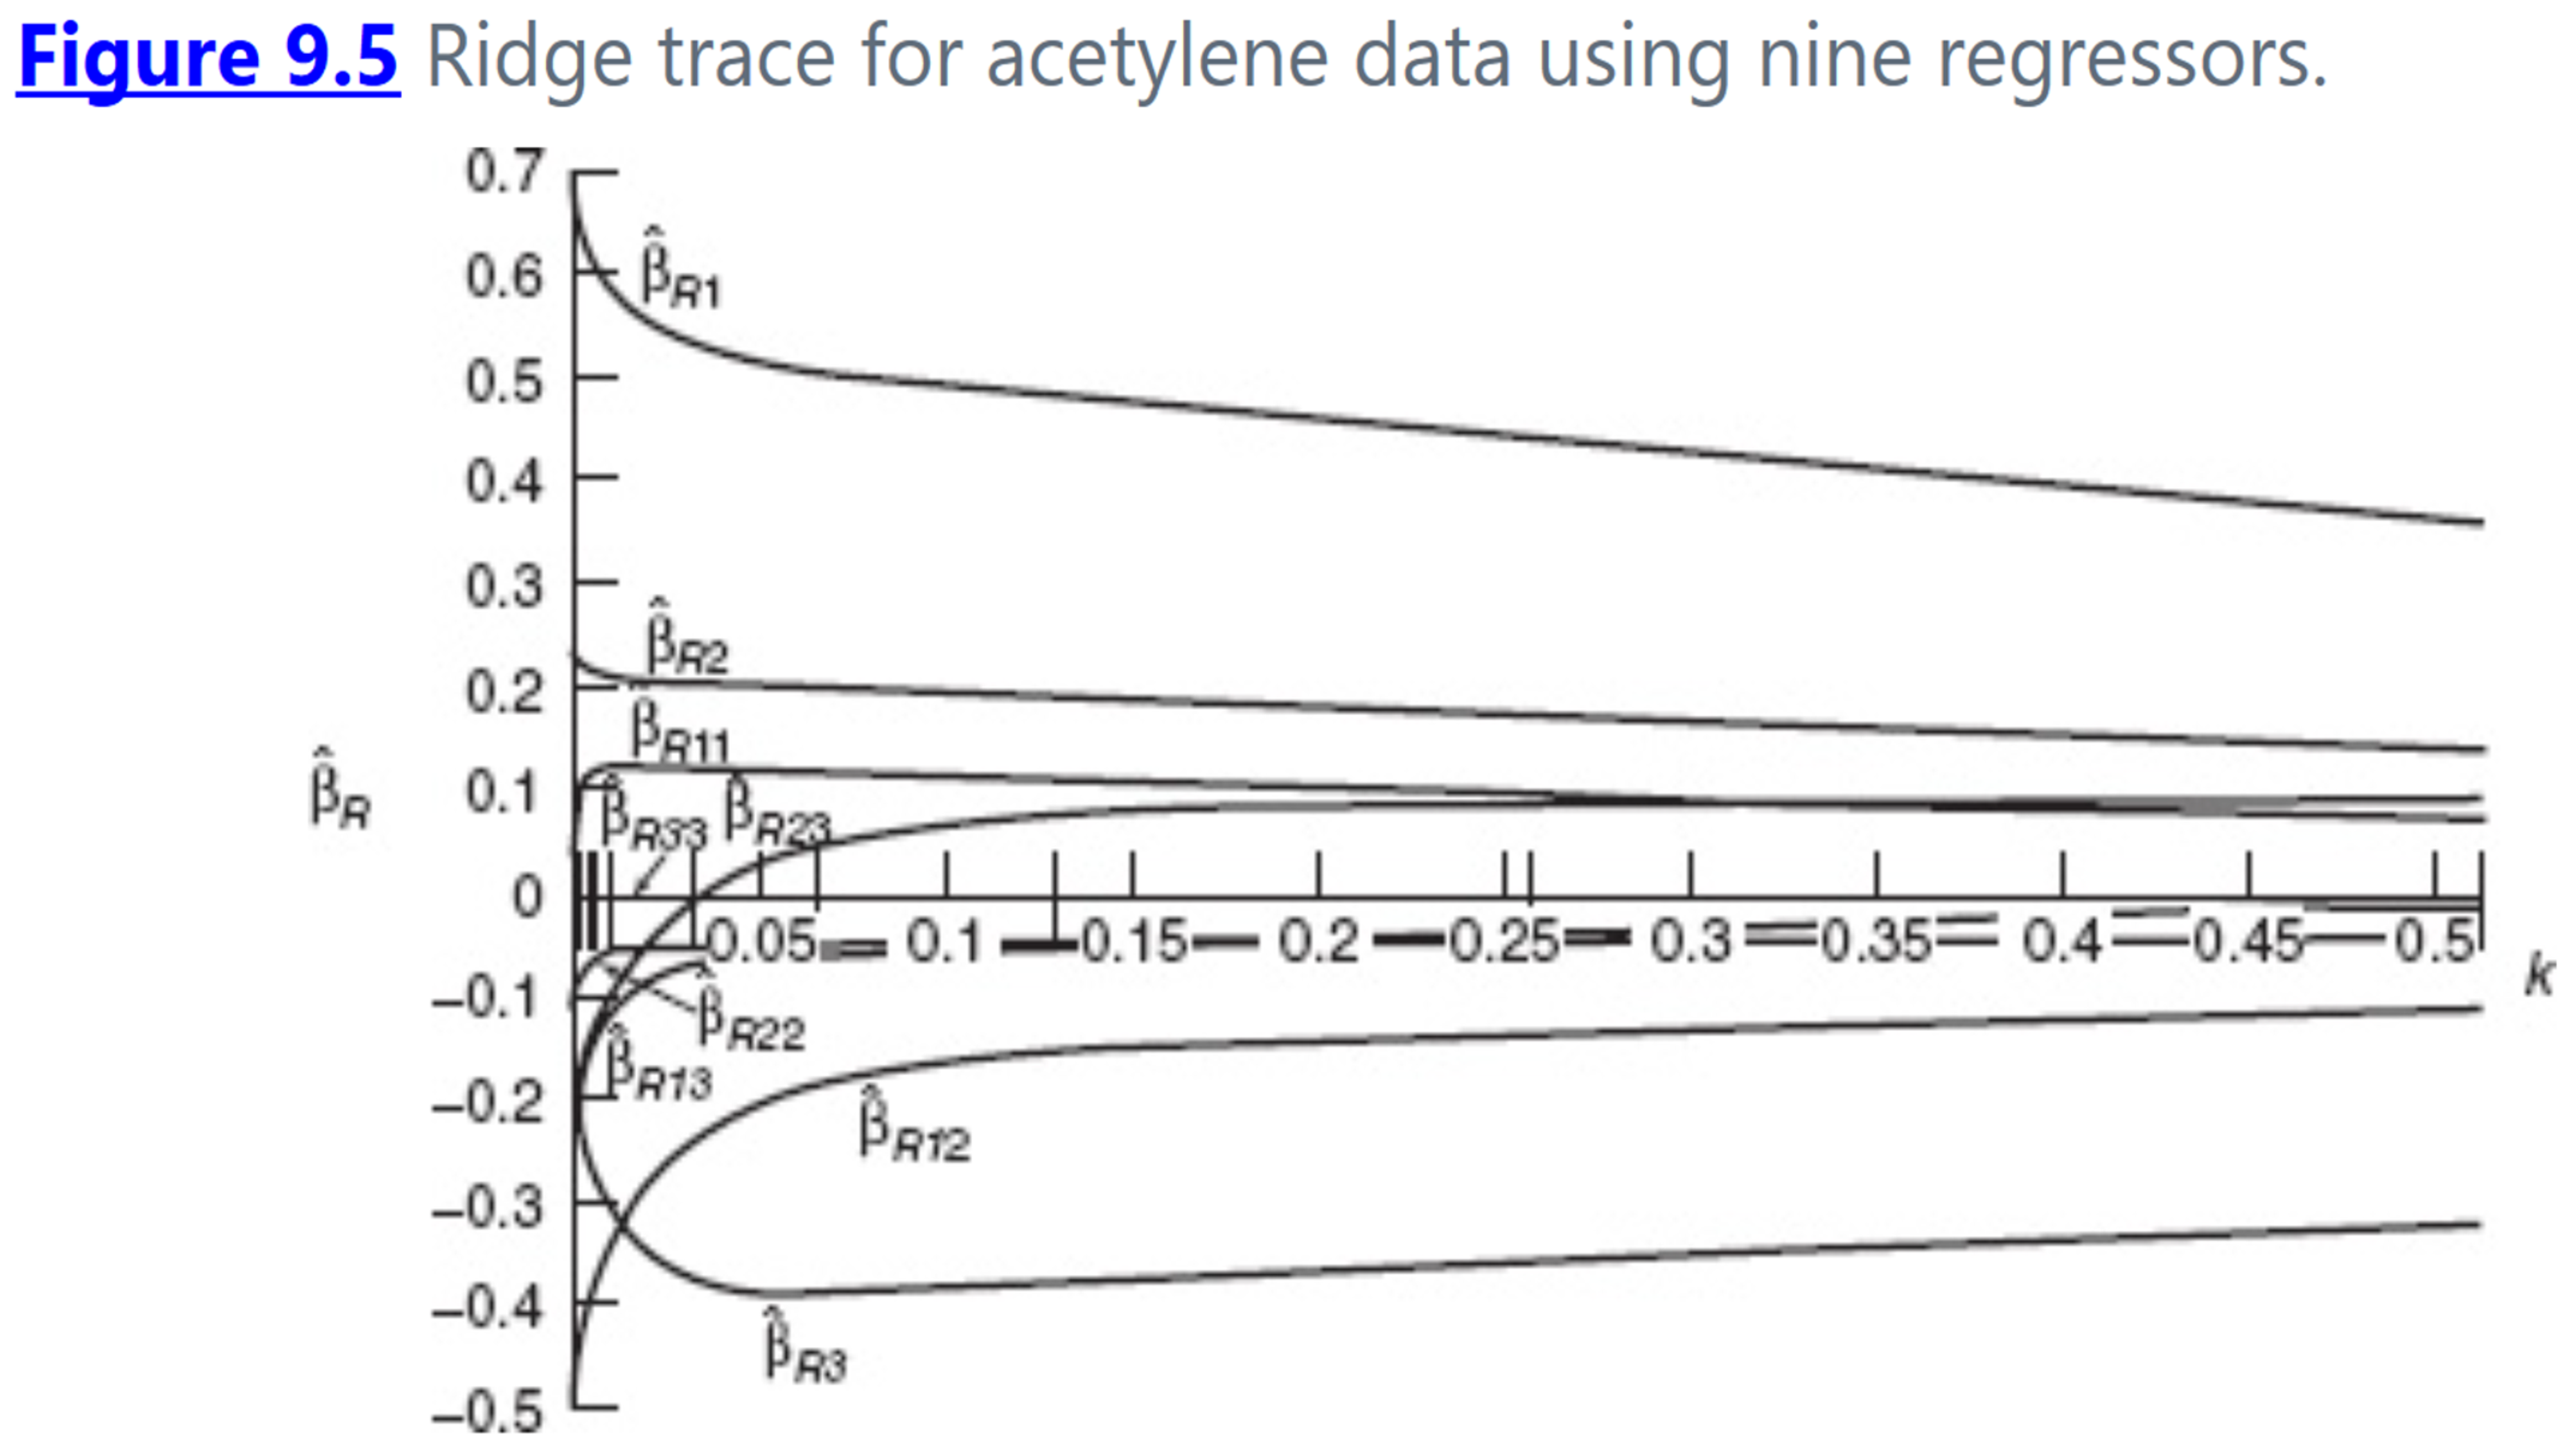
\includegraphics[width=\linewidth]{figures/ridge_trace.pdf}
            \begin{lstlisting}[language=R]
library(MASS)
# only mass
plot(lm.ridge(y~x,data=data,
        lambda=seq(0, 0.5, 0.01)))
select(model)
            \end{lstlisting}

    \section{Variable Selection}

    Basic Strategy for Variable Selection
    \begin{enumerate}
        \item Fit full model
        \item Perform analysis (full residual analysis and investigate collinearity)
        \item Determine transformation on response and some regressors
        \item Use $t$-test on individual regressors
        \item Perform analysis on edited model (esp residual analysis)
    \end{enumerate}

    \subsection{Consequence of Model Misspecfication}

    \begin{enumerate}
        \item $\hat\beta_q$ is biased for subset model
        \item $Var(\hat\beta^*_q) \geq Var(\hat\beta_q)$
        \item $MSE(\hat\beta_q^*) \geq MSE(\hat\beta_q)$
        \item $\hat\sigma$ is biased for subset model
        \item $MSE(\hat y^*) = Var(\hat y^*) \geq MSE(\hat y)$
    \end{enumerate}

        \subsection{Criteria for Evaluating Subset Regression models}

        \begin{itemize}
            \item $R^2$
                \begin{align*}
                    R^2_q = \frac{SS_{R}(q)}{SS_T} = 1-\frac{SS_{Res(q)}}{SS_T}
                \end{align*}
            \item Adjusted $R^2$
                \begin{align*}
                    R^2_{adj,p} = 1-\frac{n-1}{n-p}(1-R^2_p)
                \end{align*}
            \item $MS_{Res}$
                \begin{align*}
                    MS_{Res} = \frac{SS_{Res}(p)}{n-p}
                \end{align*}
            \item Akaike Information Criterion
                \begin{align*}
                    AIC = nlog(\frac{SS_{Res}}{n})+2p
                \end{align*}
            \item Bayesian Information Criterion (OLS) by Schwartz and Sawa
                \begin{align*}
                    BIC = nlog(\frac{SS_{Res}}{n})+plog(n)
                \end{align*}
        \end{itemize}
        AIC, BIC must be comparing the same response of the same data size

        \subsection{Computational Techniques for Variable Selection}

        \begin{itemize}
            \item Evaluating All Possible models
            \item Stepwise Regression Methods
                \subitem Forward Selection
                \subitem Backward Elimination
        \end{itemize}

        \subsubsection{Forward Selection}
        \begin{enumerate}
            \item Derived the fitted values and residuals from $\hat y = \hat \beta_0 + \hat\beta_1 x-1$ (model1)
            \item Fit the regression model: $\hat x_j = \hat\alpha_{0j}+\hat\alpha_{1j}x_1, j\in[2,k]$
            \item Derive the simple correlation between the residuals of Model 1 and the residuals from $k-1$ models above
            \item The $x_j$ that give the largest correlation will be the next regressor to enter the model
        \end{enumerate}
        Add to model if
        \begin{align*}
            F = \frac{SS_R(x_2|x_1)}{MS_{Res}(x_1, x_2)} > F_{in}
        \end{align*}
            \begin{lstlisting}[language=R]
library(leaps)
model <- lm(y~1) # only intercept
step(model, direction="forward",
            scope=y~x1+x2+x3)
            \end{lstlisting}

        \subsubsection{Backward Elimination}
        \begin{enumerate}
            \item Start model with $k$ regressor, compute partial $F$ statistic for each regressors as if it was the last varaible to enter the model
            \item regressor with the smallest F stat is examined first and removed if $F < F_{out}$
            \item Fit new model with rest of $k-1$ regressors and calculate partial F stat. Regressor with smallest partial F stat is remove if $F<F_{out}$
        \end{enumerate}
            \begin{lstlisting}[language=R]
library(leaps)
model <- lm(y~x1+x2+x3)
step(model, direction="backward")
            \end{lstlisting}

    \subsubsection{Stepwise Regression Methods}
    \begin{enumerate}
        \item At each step, all the regressors entered model previously are reassesssed via their partial F stat
        \item A regressor added at earlier step may now be redundant because of the relationship between it and regressors now in the model
        \item If the partial F stat for a variables is less than $F_{out}$ then variable is dropped from the model
        \item Stepwise regression method requires two cutoff values. One for entering variables and one for removing them. It's often $F_{in}>F_{out}$
      \end{enumerate}
      \begin{lstlisting}[language=R]
library(leaps)
model <- lm(y~x1+x2+x3)
step(model, direction="both")
      \end{lstlisting}

    \subsection{Strategy for Regression Model Building}
    Always choose the model passing model adequcy instead of just high $r^2$
    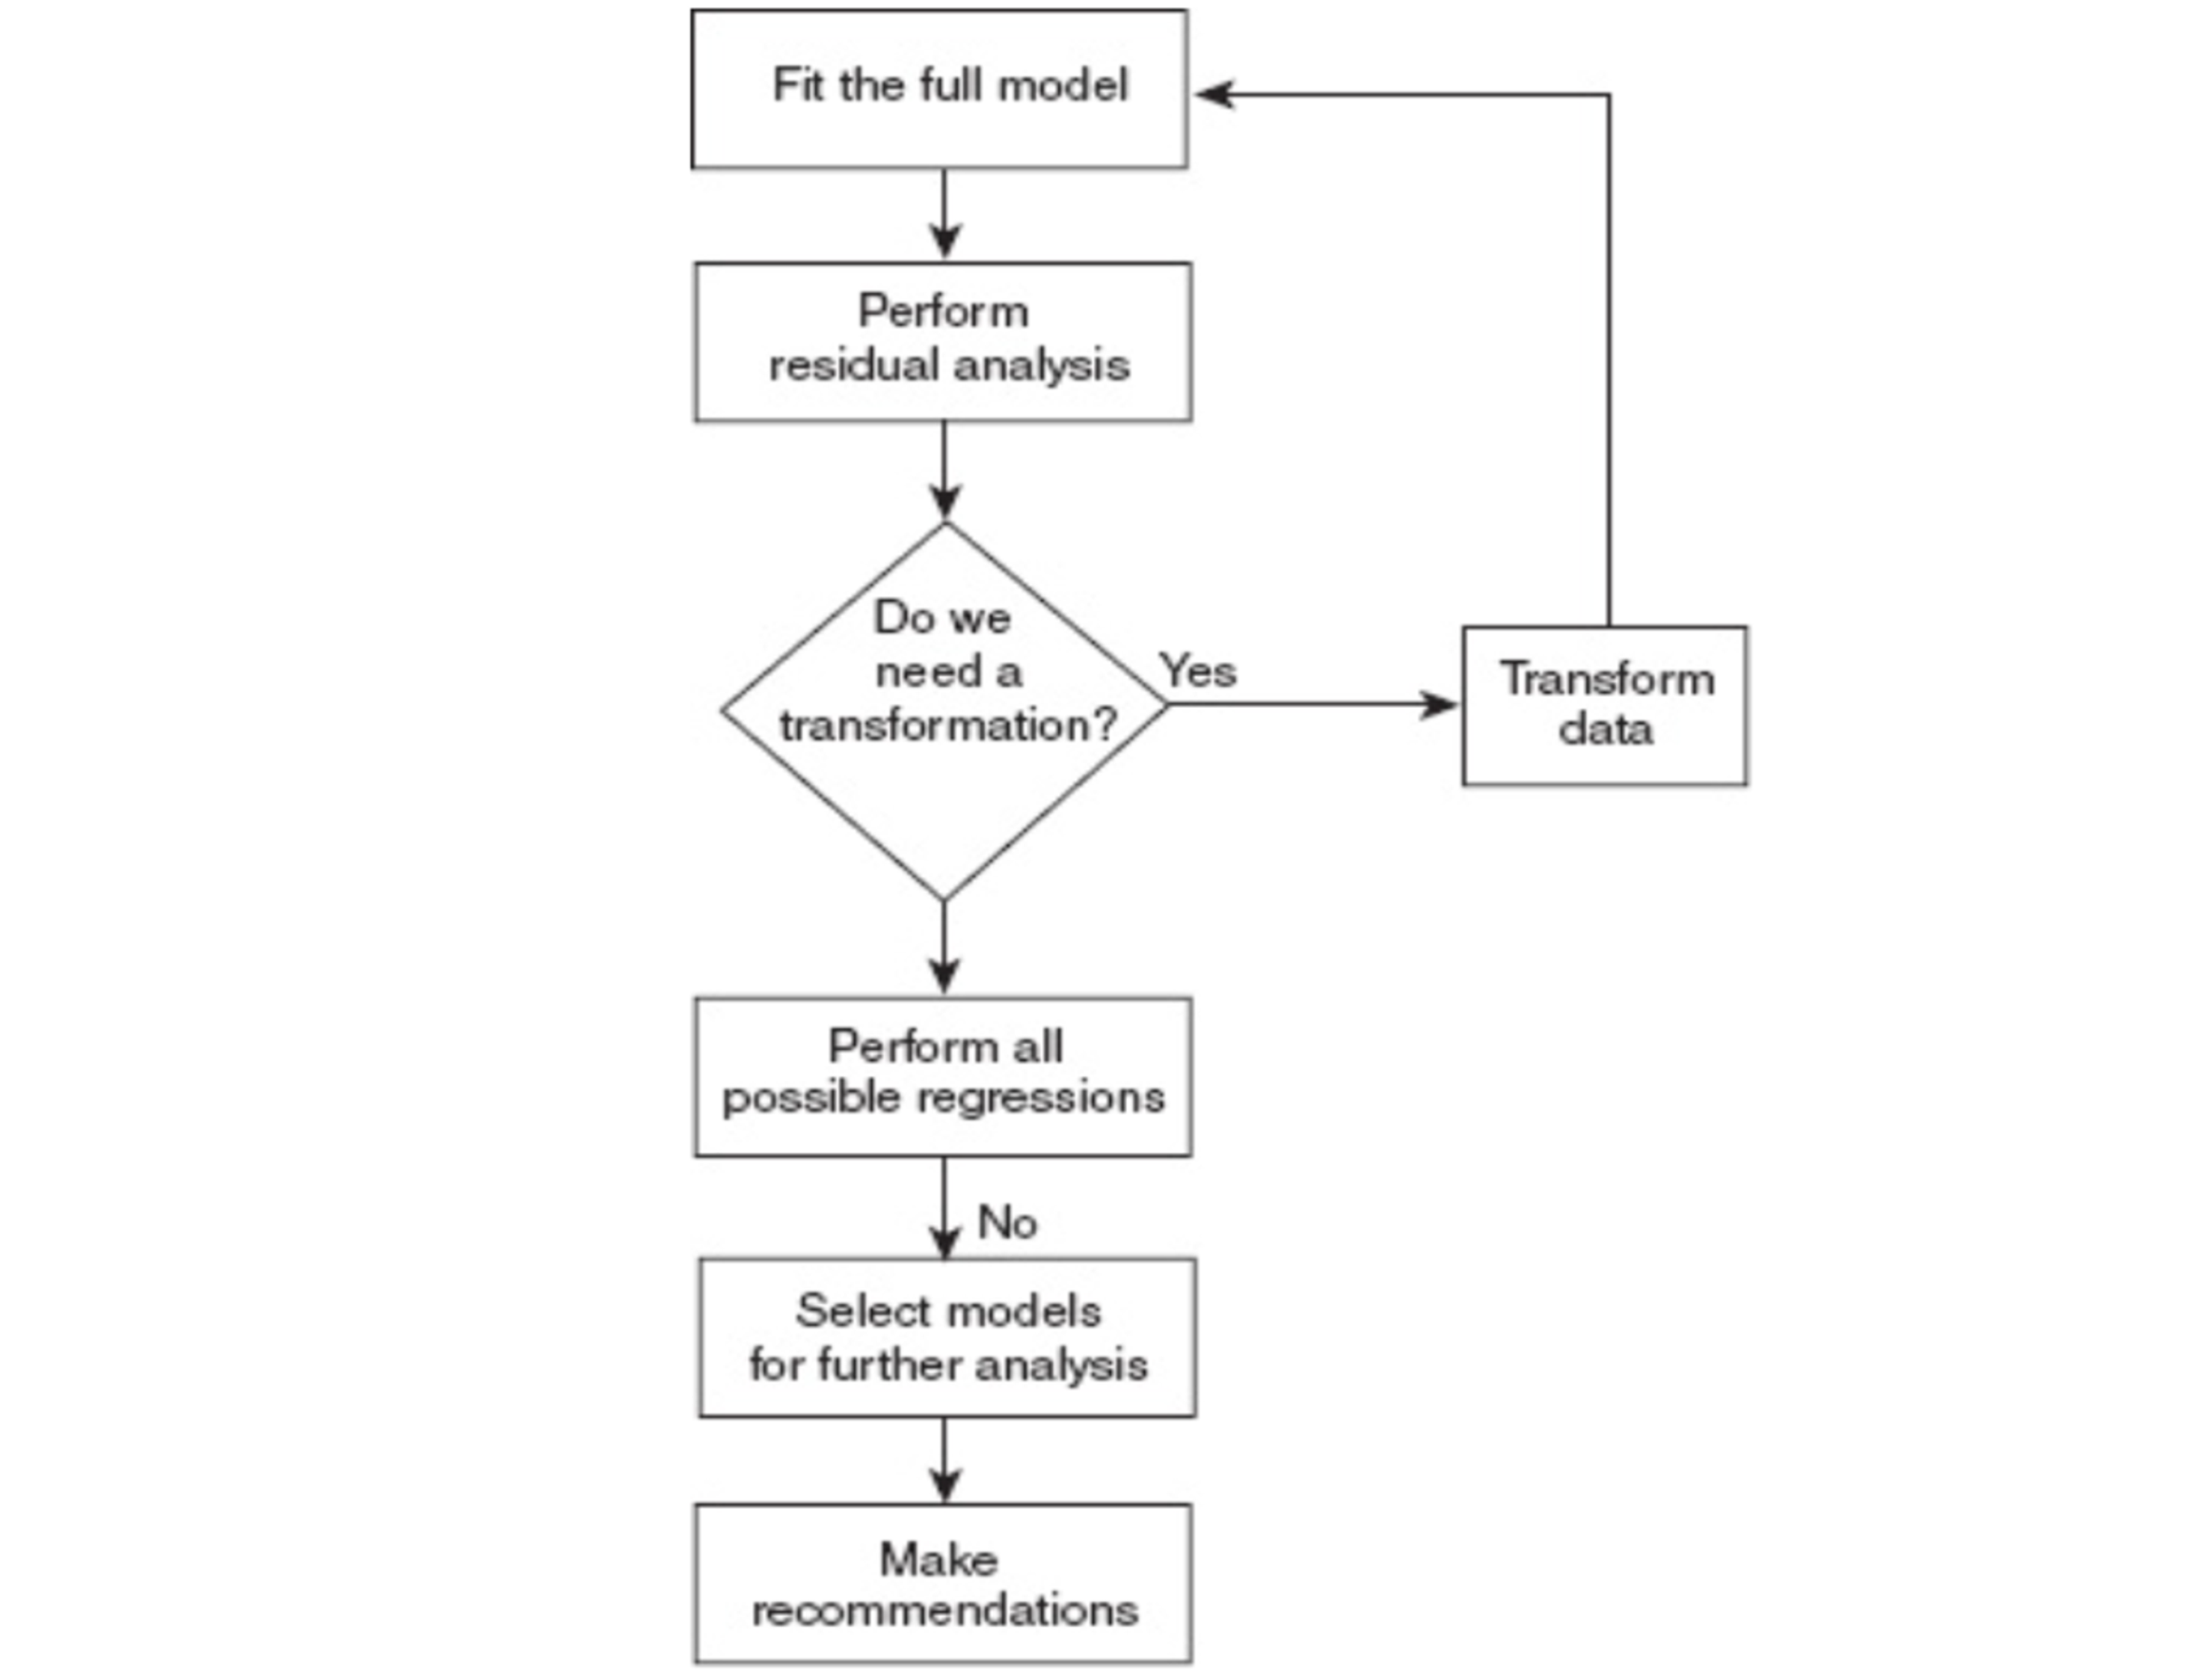
\includegraphics[width=\linewidth]{figures/lm_strategy.pdf}

\end{multicols}












\end{document}
